\documentclass[
%%%%% Styles and Sizes
%10pt,
%11pt,
%12pt,
%fancyheadings, % headings with seplines and logo
%
%%%%% Printing, Color and Binding
a4paper, 
%a5paper,
twoside, % duplex printout (default)
%oneside, % single sided printout
%% binding correction is used to compensate for the paper lost during binding
%% of the document
BCOR=20mm, % binding correction
DIV=13, % binding correction
%nobcorignoretitle, % do not ignore BCOR for title page
%% the following two options only concern the graphics included by the document
%% class
%grayscaletitle, % keep the title in grayscale
grayscalebody, % keep the rest of the document in grayscale
%
%%%%% expert options: your mileage may vary
%baseclass=..., % special option to use a different document baseclass
toc=bibliography,
numbers=noenddot, 
abstract=true
]{mtecreprt}

% Possible language options for mtec template: 'english', 'german', 'ngerman'
\usepackage[english]{babel}

% Information for the Titlepage
\author{Lennard Korte}
\title{Impact of different Data Augmentation Techniques for Deep Learning with Optical Coherence Tomography }
\date{\today}

%\degreethesisname{Computer Science}
\matriculationnumber{53673}
\studyprogram{Computer Science}

% subject can take following options:
% 'project' for 'Project Paper' or 'Projektarbeit'
% 'seminar' for 'Seminar Paper' or 'Seminararbeit'
% 'studentresearch' for 'Student Research Project' or 'Studienarbeit'
% 'diploma' for 'Diploma Thesis' or 'Diplomarbeit'
% 'degree' for 'Degree Thesis' or 'Dissertation'
% 'master' for 'Master Thesis' or 'Master-Arbeit'
% 'bachelor' for 'Bachelor Thesis' or 'Bachelor-Arbeit'
\subject{bachelor}
\degree{Bachelor of Science} % this work is for the fulfillment of the said degree
\professor{Alexander Schlaefer (Dr.-Ing.)}
\firstsupervisor{Robin Mieling (MSc.)}

\firstreferee{Prof. Dr.-Ing. Alexander Schlaefer}
\secondreferee{Till Robin Mieling (B.Sc)} 

%\company{ABC GmbH}
%\companylogofile{logo/logo_company}

\usepackage[utf8]{inputenc}

\usepackage{caption}
\captionsetup[table]{skip=10pt}

\usepackage{pgfplots}
\pgfplotsset{compat=1.16}

% Font and Fontencoding Magic
% FAQ: 
% http://tex.stackexchange.com/questions/664/why-should-i-use-usepackaget1fontenc
% http://en.wikipedia.org/wiki/Computer_Modern
% http://tex.stackexchange.com/questions/1390/latin-modern-vs-cm-super
\usepackage[T1]{fontenc}
\usepackage{lmodern}
%\usepackage{fix-cm}
\usepackage[protrusion=true,expansion=true,auto=true,tracking=true]{microtype}

% to generate some dummy text
\usepackage{lipsum}

% For graphics, graphicx package included by the class
\graphicspath{{../figures/}}

% to use Tikz for figures
\usepackage{tikz}
\usetikzlibrary{matrix,chains,positioning,decorations.pathreplacing,arrows}
\usepackage{etoolbox} % for \ifnumcomp
\usepackage{listofitems} % for \readlist to create arrays
\usepackage{pgfplots}
\usetikzlibrary{shapes,arrows,3d,calc,fit,shadows,decorations,automata,backgrounds,petri,positioning}
\usepackage{xargs}
\newcommandx*{\includetikz}[3][1=\linewidth,2=0.3\linewidth]{
 \newlength{\fwidth}
 \setlength{\fwidth}{#1}
 \newlength{\fheight}
 \setlength{\fheight}{#2}
 \input{#3}
 \global\let\fwidth\undefined
 \global\let\fheight\undefined
}
\newcommandx*{\includescaledtikz}[2][1=1]{
 \newcommand{\myscale}{#1}
 \input{#2}
}

%\usepackage[rgb]{xcolor}
\newcommand{\matr}[1]{\mathtt{#1}}     % ISO complying version
\newcommand{\vect}[1]{\bm{#1}}     % ISO complying version

% TF mat shorthand
\newcommand{\tfMat}[3]{{}^\mathrm{#1} \matr{#2}_\mathrm{#3}}
\newcommand{\invMat}[1]{\matr{#1}^{-1}}

%subcations with two images
\usepackage{subcaption}

%This is to avoid errors
\pgfplotsset{compat=1.18}

%To insert multiline comments
\usepackage{comment}

%Mathematical Letters
\usepackage{amsfonts}
\usepackage{amssymb}

%include pdf graphics
\usepackage{pdfpages}

%For ResNet18 Graphics
\usepackage[mode=buildnew]{standalone}

%use micro meter commands
\usepackage{upgreek}

%Import glossar package
\usepackage[acronym]{glossaries}
\makenoidxglossaries
\newacronym{3d}{3D}{three-dimensional}
\newacronym{2d}{2D}{two-dimensional}
\newacronym{1d}{1D}{one-dimensional}
\newacronym{ivoct}{IVOCT}{intravascular optical coherence tomographie}
\newacronym{ivus}{IVUS}{intravascular ultrasound}
\newacronym{dl}{DL}{deep learning}
\newacronym{oct}{OCT}{optical coherence tomographie}
\newacronym{td-oct}{TD-OCT}{time domain optical coherence tomographie}
\newacronym{fd-oct}{FD-OCT}{frequency domain optical coherence tomographie}
\newacronym{sd-oct}{SD-OCT}{spectral domain optical coherence tomographie}
\newacronym{ss-oct}{SS-OCT}{swept source optical coherence tomographie}
\newacronym{acc}{ACC}{accuracy}
\newacronym{bacc}{BACC}{balanced accuracy}
\newacronym{sens}{SENS}{sensitivity}
\newacronym{spec}{SPEC}{specificity}
\newacronym{ppv}{PPV}{positive predictive values}
\newacronym{npv}{NPV}{negative predictive values}
\newacronym{fdr}{FDR}{false discovery rate}
\newacronym{for}{FOR}{false omission rate}
\newacronym{roc}{ROC}{receiver operating characteristic}
\newacronym{auroc}{AUROC}{area under the receiver operating characteristics curve}
\newacronym{aupr}{AUPR}{area under precision-recall curve}
\newacronym{lnd}{LND}{line of no-discrimination}
\newacronym{mcc}{MCC}{Matthews correlation coefficient}
\newacronym{dor}{DOR}{diagnostic odds ratio}
\newacronym{resnet}{ResNet}{residual neural network}
\newacronym{nn}{NN}{neuronal network}
\newacronym{cnn}{CNN}{convolutional neural network}
\newacronym{da}{DA}{data augmentation}
\newacronym{ml}{ML}{machine learning}
\newacronym{rel}{ReL}{rectified linear activation function}
\newacronym{relu}{ReLU}{rectified linear activation function unit}
\newacronym{gan}{GAN}{generative adversarial network}
\newacronym{mse}{MSE}{mean squared error}
\newacronym{cv}{CV}{cross-validation}
\newacronym{clahe}{CLAHE}{contrast limited adaptive histogram Equalization}




\newglossaryentry{makimamethod}
{
        name=Makima method,
        text=Makima method,
        description={Is a MATLAB-specific modification of Akima's derivative formula and shortcut for modified Akima piecewise cubic Hermite interpolation}
}

\newglossaryentry{a-scan}
{
        name=A-scan,
        text=A-scan,
        description={Is a one-dimensional Depth profile}
}


\newglossaryentry{b-scan}
{
        name=B-scan,
        text=B-scan,
        description={Is a two-dimensional image, sequence of A-scans shifted along a lateral spatial dimension}
}

\newglossaryentry{c-scan}
{
        name=C-scan,
        text=C-scan,
        description={Is a three-dimensional image, sequence of B-scans shifted along third spatial dimension}
}

\newglossaryentry{m-scan}
{
        name=M-scan,
        text=M-scan,
        description={Is a two-dimensional image, but temporal sequence of A-scans}
}

\newglossaryentry{batch-normalization}
{
        name=Batch normalization,
        text=batch normalization,
        description={Is a method of making artificial neural networks faster and more stable by normalizing layer inputs through rescaling and rescaling}
}

\newglossaryentry{regression}
{
        name=Regression,
        text=regression,
        description={Is a statistical method that attempts to assess the strength and character of the relationship between a dependent variable and a set of other variables \cite{Beers.2021}}
}

\newglossaryentry{logistic-regression}
{
        name=Logistic regression,
        text=logistic regression,
        description={Is a technique for modeling the probability of a discrete outcome as a function of an input variable. The most common logistic regression models a binary outcome with help of the Sigmoid function in contrast to linear regression often used for continuous variable estimation \cite{Edgar.2017}}
}

\newglossaryentry{overfitting}
{
        name=Overfitting,
        text=overfitting,
        description={Is a modeling error in statistics that occurs when a function is too closely aligned to a limited set of data points. As a result, the model is useful in reference only to its initial data set, and not to any other data sets. \cite{Twin.2021} In Machine Learning it refers to high error with respect to test data as well as low prediction error with respect to training data}
}

\newglossaryentry{generalizability}
{
        name=Generalizability,
        text=generalizability,
        description={Generalization refers to your model's ability to adapt properly to new, previously unseen data, drawn from the same distribution as the one used to create the model \cite{GoogleDevelopers.2022}}
}

\newglossaryentry{heat-map}
{
        name=Heat map,
        text=heat map,
        description={Is a representation of data in the form of a map or diagram in which data values are represented as colors \cite{OxfordUniversityPress.2022}}
}

\newglossaryentry{optimizer}
{
        name=Optimizer,
        text=optimizer,
        description={Is an algorithm that modifies the weights, biases and learning rate of a neural network to minimize the cost function (or error) and thus improves prediction performance. Thus, its choice is a key aspect in having a successful training of a NN}
}

\newglossaryentry{learning-rate}
{
        name=Learning rate,
        text=learning rate,
        description={Is a hyper parameter that controls how much weights and biases of a neural network are adjusted during training with respect to the error gradient}
}

\newglossaryentry{debian}
{
        name=Debian,
        text=Debian,
        description={Is a free and open-source Linux distribution, usually known as Debian GNU/Linux, that was created by the community-supported Debian project, founded by Ian Murdock}
}

\newglossaryentry{wrs}
{
        name=Weighted random sampler,
        text=weighted random sampler,
        description={Is a sampling algorithm, that is able to select a sample from a given data set subdivided into k classes. The specified selection probabilities can be unequally distributed such that one can counteracting imbalances for further processing}
}

\newglossaryentry{wandb}
{
        name=WandB,
        text=WandB,
        description={Is a central dashboard that allows you to keep track of your hyperparameters, system metrics, and forecasts in real time, allowing you to observe and compare models in real time}
}

\newglossaryentry{imagenet}
{
        name=ImageNet,
        text=ImageNet,
        description={Is a large visual database designed by a number of academic contributors for use in visual object recognition software research}
}

\newglossaryentry{deepcopy}
{
        name=Deep Copy,
        text=deep copy,
        description={Is an object that does not share the same reference as the object from which the copy was made, but has the same underlying values}
}

\newglossaryentry{affinetransformation}
{
        name=Affine transformation,
        text=affine transformation,
        description={Is a geometric transformation that does not necessarily preserve distances and angles, but lines and parallelism}
}

\newglossaryentry{atherosclerosis}
{
        name=Atherosclerosis,
        text=atherosclerosis,
        description={Is the thickening or hardening of the arteries, that is caused by a buildup of plaque in the inner of an artery}
}

\newglossaryentry{interpolation}
{
        name=Interpolation,
        text=interpolation,
        description={Is a method of finding new data points based on the range of a discrete set of known data points. To generate a simplified function that is still quite close to the original a data points from the original function are interpolated}
}

\newglossaryentry{histogram}
{
        name=Histogram,
        text=histogram,
        description={Is a graphical representation of the images intensity distribution. It visualizes the number of pixels for each intensity value}
}

\newglossaryentry{mutualinformation}
{
        name=Mutual information,
        text=mutual information,
        description={Is a measure of image matching, that expresses the amount of information given by image Y on image X. A value of 1.0 would reflect perfect agreement and 0.0 complete disagreement between the two images X and Y.}
}


%Import multirow package for Table
\usepackage{multirow}

\begin{document}
\frontmatter
\maketitle
\tableofcontents

% Add to table of contents
\cleardoublepage
\addcontentsline{toc}{chapter}{\listfigurename}
\listoffigures{}

\let\cleardoublepage\clearpage

\begingroup
\let\clearpage\relax
% Add to table of contents
\cleardoublepage
\addcontentsline{toc}{chapter}{\listtablename}
\listoftables{}
\endgroup

% Add to table of contents
\cleardoublepage
\addcontentsline{toc}{chapter}{\acronymname}
\printnoidxglossary[type=\acronymtype]
\newpage
\begingroup
\let\clearpage\relax
% Add to table of contents
\cleardoublepage
\addcontentsline{toc}{chapter}{\glossaryname}
\printnoidxglossary
\endgroup

\chapter{Abstract}

\Gls{atherosclerosis} is one of the leading but preventable and treatable causes of death worldwide. For effective treatment, e.g. choice of stent size and its positioning, it is essential for the attending physician to have an accurate idea of the intravascular anatomy. Lesions (plaque) and arterial walls can be visualized with \acrfull{ivoct}, a high-resolution imaging technique, that can be applied by experts. Due to the high number of images captured during clinical routines, research spends tremendous efforts on automatic plaque detection (image classification) with \acrfull{dl} in polar as well as cartesian representation for fast and accurate decision support. \Acrfull{da} is an essential part of training \acrshort{dl} models in machine learning. A variety of augmentation strategies, including cropping, flipping, and convolutional filters, have been proposed. They have shown to maintain important characteristics of \acrshort{ivoct} images without handcrafting features, especially when in cartesian representation. While data augmentation has been commonly used for deep learning in \acrshort{ivoct} imaging, little work has been done to determine which augmentation techniques capture medical image statistics best and lead to a higher model performance. This work provides an overview about conventional techniques and proposes new, advanced techniques tested on a data set consisting of labeled in vivo patient images. Furthermore, augmentation techniques are compared and those that add value are proposed for further investigation building domain specific training strategies. Finally, it was shown that the models performance is determined by the extent to which relevant information and features of the original medical images are preserved in the augmented training sets. Overall, we find that a model trained with data that are augmented by the discussed techniques, for instance shifting or shearing, may boost the performance by 0.05 in \acrfull{mcc} and 0.03 in \acrfull{bacc}. On the other hand, less effective transformations such as contrast jittering may deteriorate scores significantly by more than ten percent. Our results show that the right \acrshort{da} strategy is essential for performance optimization when building deep learning-based clinical decision support systems for plaque detection.




\mainmatter
\chapter{Introduction}

% Hinführung
Coronary heart disease is one of the leading causes of death \cite{HannahRitchie.2018, NationalVitalStatisticsReports.2017} accounting for more that 15\% of all deaths in 2015 \cite{Kolluru.2018}, despite being preventable and treatable. To treat the causes of coronary heart disease, \acrfull{oct} technology can be used to allow a detailed examination of the in vivo tissue anatomy and coronary procurement from within.

% (IV-)OCT
In comparison to the typically used \acrfull{ivus} technology, \acrfull{ivoct} offers a higher micrometer resolution utilizing interferometry low-coherent light \cite{Schippling.2015, Drexler.2008}. Both imaging techniques that can be used for planning stent interventions or during interventions to guide stent placement and characterize atherosclerotic plaque types \cite{Kolluru.2018}. \Acrshort{ivoct} is well suited for embedding in thin medical instruments such as catheters, because the infrared light can be transmitted via glass fibres \cite{HiramG.Bezerra.2009, Gessert.2019}. Due to its low penetration depth capabilities, it only allows visualization of regions directly around the catheter. This is sufficient for the attending physicians to obtain a detailed understanding of the region of interest, i.e. the arterial obstruction. \cite{Gessert.2019} Currently \acrshort{ivoct} is the only imaging technique that enables identification of the most rupture susceptible thin-cap fibroatheroma \cite{GuhaRoy.2016}.

% Why automatically?
A key problem is the large number of frames (often > 500) arising from single 2s to 5s pullbacks in \acrshort{ivoct} interventions \cite{Kolluru.2018}, that cannot be reviewed by the practitioner during clinical routine. Automatic plaque detection is of major importance for a fast and accurate decision support system \cite{Gessert.2019}. These must offer reliable information on the presence and nature of stenosis \cite{Gessert.2019}. Various approaches for automatic \acrshort{ivoct} data analysis have been proposed. Correlating the images to histology data proofs general feasibility of inferring plaque characteristics from \acrshort{ivoct} data \cite{Yabushita.2002}.

% bisherige forschung
Methods for automatic \acrshort{ivoct} data analysis like stent detection \cite{Zhao.2015, Lu.2012} and automatic lumen segmentation \cite{GuhaRoy.2016, Tsantis.2012} have been proposed. Automatic classification approaches using texture and optical properties as features have been proposed for plaque detection and segmentation \cite{Ughi.2013, Celi.2014}. \Acrshort{dl} approaches have been proposed more recently for \acrshort{ivoct} data processing \cite{Abdolmanafi.2017}, in particular \acrfullpl{cnn} have shown remarkable success in image analysis tasks such as segmentation \cite{Long.2015} and classification \cite{Gessert.2018}. Even if plaque detection with \acrshortpl{cnn} has been employed mostly in preliminary studies, they provide promising initial results. Recent standard architectures such as Inception or \acrfullpl{resnet} have shown significant performance improvement for medical image analysis \cite{Long.2015, Gessert.2018}. The approach using \acrshort{cnn}s in medical diagnostic tasks offers the advantage that we can omit the complicated and error-prone step of tissue segmentation. Progress has been made in using \acrshort{dl} for image classification, especially in the prediction and segmentation of cancerous masses in lung, liver or breast scans \cite{Cho.2015, CruzRoa.2013, Fakoor.2013}.

% DL challenges
Nevertheless, various shortcomings still need to be addressed. Polar images are often converted to cartesian representation for easier and more intuitive interpretation by practitioners. One of the questions that remains unanswered is whether either or both images (e.g. in two path \acrfull{dl} architectures) are the more advantageous choice for training the \acrshort{dl} models \cite{Gessert.2018} and relevant for future use. 
The lack of large labeled image data sets from \acrshort{ivoct} interventions is one of the major challenges in the process of creating \acrshort{dl} models that achieve the desired and necessary performance. Nevertheless the effect of having only a limited number of scans can be mitigated by a number of methods to a certain extend, for instance normalization or dropout that prevent the model from \gls{overfitting}. \Acrshort{da} denotes one of the advanced techniques that allow \acrshort{dl} models to extract features from small data sets more effectively.

Hence, the main objective of this bachelor’s thesis was to implement a \acrshort{dl} pipeline to investigate the effects of \acrshort{da} techniques tailored to polar as well as cartesian representation. It was examined which \acrshort{da} techniques have positive effects on the overall model performance, that is, the extent to which augmented data sets retain properties of the original medical images. By conducting a number of experiments we investigate which \acrshort{da} techniques are recommended to use. Their individual as well as combined performance impact on the \acrshort{cnn} has been investigated to form a strategy applicable in the domain of \acrshort{ivoct} imaging. In addition, the question is answered to what extent data augmentation techniques applied on \acrshort{ivoct} data can improve the networks performance. New \acrshort{ivoct} specific \acrshort{da} techniques are presented and included in the analysis. It is assumed that \acrshort{ivoct} images do not vary in their fundamental structure, such that observations can be transferred to other \acrshort{ivoct} data sets. Trained experts labeled the frames of each pullback with binary class characterizations that distinguished between the presence and absence of plaque.

\chapter{Theoretical Concepts}

In the following fundamental concepts of the underlying experiments are described and explained in detail. Beginning with the general concepts of image acquisition with \acrshort{ivoct}, we continue by laying out how \acrshort{dl} models work. It is explained how the behaviour and performance of utilized \acrshortpl{resnet} may be interpreted. In addition to that, an overview of frequently used \acrshort{da} techniques is provided in the context of \acrshort{dl} with \acrshort{ivoct} data.

\section{Optical Coherence Tomography}

\acrshort{oct} is a medical imaging technique for translucent or opaque materials. It works by generating an interference pattern between light traveling through the sample arm and light propagating in the reference arm of an interferometer to measure the time-of-flight of light returned from tissue \cite{AdamM.Zysk.2007, Drexler.2008}.

In an early stage \acrshort{oct} images were applied to display retinal structures, but later it was also employed in diverse applications like ophthalmology, where it is used to obtain detailed images from within the retina, and optometry for painting analysis \cite{AdamM.Zysk.2007, Drexler.2008}. Oncology and dermatology are other common areas where \acrshort{oct} is used primarily for cancer detection \cite{Welzel.2001, AdamM.Zysk.2007}. In cardiology it helps to diagnose and treat coronary artery diseases \cite{HiramG.Bezerra.2009}. Technologies like medical ultrasonography, confocal microscopy, magnetic resonance imaging and \acrshort{oct} are differently suited for morphological tissue imaging. They primarily differ in resolution and depth of view. \Acrshort{oct} has achieved a high micrometer resolution (less than \( 10 \upmu \)m axially and \( 20 \upmu \)m laterally) \cite{RighabHamdan.2012, GuillermoJ.Tearney.2012, HiramG.Bezerra.2009, KostadinkaBizheva.2017}. It allows a penetration depth of a few millimeters below the surface in biological tissue \cite{AdamM.Zysk.2007, Drexler.2008}. This is because the proportion of escaping light without scattering becomes too low in deeper sample layers so that it can be extracted \cite{Bille.2019, Drexler.2008}. Other key advantages are the ability to rapidly acquire live images directly without preparation or direct contact to the subject. Furthermore \acrshort{oct} is non invasive and non ionizing \cite{Hee.1995}.

\subsection{Principle}

\acrshort{oct} employs near-infrared light with long wavelength generated by super-luminescent diodes, which allows it to penetrate into the scattering medium. The architecture illustrated in \cref{fig:octarchitecture} is based on low-coherence interferometry (Michelson interferometer) owing to the use of light with broad bandwidths \cite{Drexler.2008, HiramG.Bezerra.2009}. The optical setup typically consists of the components described as follows. Initially, light from the source is split into two beams, first the sample arm targeted at object of interest, and second, a reference arm with a mirror. The combination of light reflection from both arms generates an interference pattern. Depending on the sample properties, areas with greater light reflection will create greater interference and vice versa. Interferometry allows direct detection of reflections, considering that the speed of light is too fast to measure it directly. The low coherence characteristic of the source light will ensure that reflections outside the coherence length will not interfere \cite{Bille.2019}. Measuring reflection intensities enables the location of structures in spacial dimension of the axial depth scan (\Gls{a-scan}). When plotting an \Gls{a-scan} against the additional time dimension, we refer to it as \Gls{m-scan}. By adjusting the sample beam position we combine multiple \Glspl{a-scan} to a series resulting in a cross-sectional tomogram referred to as \Gls{b-scan} (\acrshort{2d}) or \Gls{c-scan} (\acrshort{3d}), see \cref{fig:scanpol}. \cite{Drexler.2008, Bille.2019}
\begin{figure}
  \centering
  \includegraphics[width=\textwidth]{../figures/oct/architecture_plain.pdf}
  \caption[\acrshort{oct} architecture]{Basic architecture of an \acrshort{fd-oct} system with a Michelson interferometer \cite{Drexler.2008} at its core. The sample arm has been extended by a probe guided by the catheter and directs its beam on to a tissue \cite{Bahoshy.2022}.  }
  \label{fig:octarchitecture}
\end{figure}

Time domain \acrshort{oct} (\acrshort{td-oct}) image acquisition is highly limited in recording speed due to its scanning rate. By moving the mirror and thus changing its path length in the reference arm a reflective profile of the sample can be scanned \cite{Drexler.2008}. The later introduced frequency domain \acrshort{oct} (\acrshort{fd-oct}) with a fixed mirror offers higher sampling rate and increased sensitivity \cite{Stifter.2007}. \acrshort{fd-oct} resolves different axial positions based on the interference spectrum acquired with spectrally separated detectors. An increasing number of detection elements reduces losses and signal to noise ratio proportionally. While the scanning range is limited by parallel detection of multiple wavelength ranges, the spectral bandwidth defines the axial resolution. \cite{Gonzalo.2010} We further distinguish between the two specialisations: spectral domain \acrshort{oct} (\acrshort{sd-oct}) and swept source \acrshort{oct} (\acrshort{ss-oct}). \acrshort{sd-oct} utilizes a broad light source with a spectrometer measuring all echo times simultaneously. Echo intensity distribution is resolved in space rather than in time \cite{Kalkman.2017}. An \Gls{a-scan} is made up by the accumulation of all axial measurements of the echo time delay. Special dispersive detectors are used to separate wavelengths. \cite{Bille.2019} In contrast \acrshort{ss-oct} encodes optical spectral frequency generated by a swept source laser. This enables the spectral measurement over time acquired by a spectral scanning source. Other known approaches are line field \acrshort{oct} using a broadband laser and line detection camera \cite{ArnaudDubois.2018, Ruini.2021} and full field \acrshort{oct}, where images are acquired orthogonal to the light beam of illumination \cite{E.Beaurepaire.1998}.

Subsequently, we describe the axial ranging with low-coherence interferometry analogous to Drexler \cite{Drexler.2008}. The following abstract will give an introductory overview of the most fundamental concepts in \acrshort{oct} technology. They have been described in papers by Billie and Drexler in detail \cite{Bille.2019, Drexler.2008}. Assuming a known spectrum of the light source, with wavenumber \( k \) and an angular frequency of the light source, we can determine the samples reflective properties. The electrical field at time \( t \) and distance \( z \) with field amplitude \( s(k,w) \) is defined as
\begin{equation}
    E_i = s(k,w)e^{i(kz-wt)}.
    \label{eq:energylightsource}
\end{equation}
The wavelength-independent beam splitter with a ratio of 0.5 ideally splits the source light into two equal parts. With a reflector distance to the beam splitter of \( z_R \) and a electric field reflectivity of \( r_R \), the returned energy can be described as:
\begin{equation}
    E_R = \frac{E_i}{\sqrt{2}}r_R e^{i2kz_R}.
    \label{eq:energyreflector}
\end{equation}
The sample has a depth dependent and continuous electric field reflectivity profile \( r_s(z_s) \). Note that \( z_s \) denotes the pathlength variable from the beam splitter along the beam axis. The reflected energy can be described with a convolution (\( * \)) by:
\begin{equation}
    E_S = \frac{E_i}{\sqrt{2}} \left[ r_S(z_S) * e^{i2kz_S} \right]
    \label{eq:energysample}
\end{equation}
For illustrative purposes we describe the sample reflection properties as a layered model \( r_S \). Thus, we abstract it as series of \( N \) discrete real delta functions of the form
\begin{equation}
r_{\mathrm{S}}\left(z_{\mathrm{S}}\right)=\sum_{n=1}^{N} r_{\mathrm{S} n} \delta\left(z_{\mathrm{S}}-z_{\mathrm{S} n}\right)
\label{eq:layered}
\end{equation}
Furthermore we have \( r_{Sn} \) as electric field reflectivity and \( z_{Sn} \) as pathlength from the beam splitter at layer \( n \). After the returning fields passed through the beamsplitter a second time, their power is halved. They interfere at the square-law detector that generates a photocurrent according to its responsivity \( \rho \):
\begin{equation}
    I_D(k,w) = \frac{\rho}{2}\bigg\langle \bigg| \frac{s(k,w)}{\sqrt{2}}r_R e^{i(2kz_R-wt)} + \frac{s(k,w)}{\sqrt{2}} \sum^N_{n=1}r_{Sn}e^{i(2kz_{Sn}-wt)} \bigg|^2 \bigg \rangle .
    \label{eq:msf}
\end{equation}
Taking into account that a detector in praxis is not able to detect the temporal angular frequency \( w \) due to its response time, we can neglect the temporal invariant terms. With the help of the Eulers rule and by substituting the power spectral dependence of the light source \( S(k) = \langle \left| s(k,w) \right|^2 \rangle \), the equation can then be rewritten as a sum of three components:
\begin{equation}
\begin{aligned}
    I_D(k) & = \frac{\rho}{4} \left[ S(k) \left( R_R + \sum^{N}_{n=1} R_{Sn}\right) \right] \text{DC Terms,} \\
           & + \frac{\rho}{2} \left[ S(k)\sum^N_{n=1} \sqrt{R_R R_{Sn}} \left( \cos [2k(z_R - z_{Sn}] \right) \right] \text{Cross-correlation Terms and} \\
           & + \frac{\rho}{4} \left[ S(k)\sum^N_{n \ne m = 1} \sqrt{R_{Sn} R_{Sm}} \left( \cos [2k(z_{Sn} - z_{Sm}] \right) \right] \text{Auto-correlation Terms}
    \label{eq:untuitiveform}
\end{aligned}
\end{equation}

First, the DC term depends on power reflectivity of the mirror and is proportional to the source wavenumber spectrum. Sample reflectivity information are provided by the cross-correlation term. It depends on the pathlength difference between sample reflectors and reference arm, as well as the light source wavenumber and contains the desired reflection profile information. Additionally the often comparatively small autocorrelation term represents artifacts created by interference occuring between sample reflectors. 

Note that the light source spectrum \( S(k) \), characterized by the wavenumber bandwidth \( \delta k \), is the inverse of the Gaussian-shaped coherence function \( y(z) \) characterized by the coherence length \( l_c \). The coherence length is a function of the light source bandwidth. \cite{Kalkman.2017}
\begin{equation}
l_{c}=\frac{2 \sqrt{\ln (2)}}{\Delta k}=\frac{2 \ln (2)}{\pi} \frac{\lambda_{0}^{2}}{\Delta \lambda}
\label{eq:wavenumberlength}
\end{equation}

\subsection{Image Reconstruction}

The raw detector signal can be reconstructed by first subtracting the known sensor specific offset and removing the DC term, which can be determined before actual measurement. In \acrshort{td-oct} the wavenumber-dependent detector current is captured on single receiver. Thus we obtain the result by integrating at each reference beam length \( k_Z \) over all k. In comparison, \acrshort{fd-oct} detects the spectral signal  \( I_D(k) \) and acquires the depth information by applying the Fourier transformation. The inverse Fourier transform should map a signal from wavenumber \( k \) to physical distance \( z \), but spectral decomposition is not necessarily linear in k-space. Therefore interpolate the wavenumber to new coordinates, also referred to as dechirping. The spectrum is linearized by mapping to corresponding non-linear and equidistant \gls{interpolation} intervals. We multiply the signal with a Hann-window to proportionally reduce the lateral deflections minimizing spectral leakage (apodisation). For interpretation as image, the complex magnitude or depth of the interferometric signal is considered, that is often logarithmically compressed. By applying the inverse Fourier transformation to the source spectrum, we obtain the desired depth information. This so called \acrshort{oct} \Gls{a-scan} with grey-scaled intensity data represents the scanned structures. The resolution is given by the coherence length along the depth axis. Laterally, the shape of the light beam is determined by the optical setup. The complex valued signal can be represented by normalizing the complex valued signal to the amplitude
\begin{equation}
\left| i(z) \right| = \sqrt{\operatorname{Re}^{2}\{i(z)\}+\operatorname{Im}^{2}\{i(z)\}}.
\end{equation}

\subsection{IVOCT}

\begin{figure}[hbt]
    \centering
    \includegraphics[width=11cm]{../figures/oct/ivoct_plain.pdf}
    \caption[\acrshort{ivoct} catheter in vessel]{Cross-sectional view showing a probe inside a catheter with a rotational pull-back as part of an \acrshort{ivoct} system. Between every A-scan, the probe rotates by an angle of \( \beta \). Optimally smaller angles allow for a higher lateral resolution of the image (for illustrative purposes here transformed to the cartesian coordinate system).}
    \label{fig:ivoct}
\end{figure}
Cardiovascular or intravascular \acrshort{oct} is a catheter based imaging technique of in vivo coronary arteries and deployed stents (see \cref{fig:octarchitecture}). It serves as a special form of \acrshort{oct} and was established as a high definition alternative to intravascular ultrasound with a slightly shorter field of view \cite{IkKyungJang.2002, GuillermoJ.Tearney.2012}. Semi-automated imaging analyses permits acquisition of a number of accurate measurements like stent apposition and neointimal thickening that can assist cardiologists while planning or executing interventions \cite{HiramG.Bezerra.2009}. Since coronary heart disease is one of the most common treatable and preventable causes of death, there is a strong demand for reliable treatment methods. \Acrshort{ivoct} can be used by experts to detect and characterize lesions and plaque deposits on the arterial wall. In practice hundreds of images are acquired in each recording raising the demand for automatic decision support for plaque detection. \Acrshort{ivoct} requires a single fiberoptic wire at the sample arm that emits light from the source and records its reflection. \cite{HiramG.Bezerra.2009} The light is guided through the probe which itself is placed inside the catheter with 0.8 to 1.0 mm diameter \cite{HiramG.Bezerra.2009}. At the tip of the probe is a prism positioned that redirects the beam focused with a given angle directly on the object of interest, i.e. an inner vessel wall. The axial resolution is determined by the light source wavelength of \( 1,250 \text{ to } 1,350 nm \) \cite{HiramG.Bezerra.2009}. Lateral resolution is determined by the spot size focused with the spot arm lens (see \cref{fig:ivoct}). The wire simultaneously rotates while being pulled back along the artery at calibrated distances. We note that only the speed of light (\(3 \times 10^8 m/s\)) enables accurate measurements when concurrently moving the wire in space with a comparatively slow speed \cite{HiramG.Bezerra.2009}. A frequency domain \acrshort{oct} system can reach pullback speeds of up to 20 millimeters per second and a rotation rate of up to 200 frames per second \cite{HiramG.Bezerra.2009}. With a penetration depth of one to three millimeters, multiple axial \Glspl{a-scan} can be continuously acquired by reflections recorded from the vessel wall (assuming a blood free environment) \cite{Gessert.2018}. Recent versions of \acrshort{ivoct} make use of \acrshort{fd-oct} (instead of \acrshort{td-oct}) with a fiberoptic coupler similar to a beam splitter. \Acrshort{fd-oct} enables us to circumvent the limitations of generating a fast optical mirror delay. Thus we can reach a significantly higher imaging frequency with up to 100 frames per second. \cite{HiramG.Bezerra.2009, Gessert.2019}

\section{Machine Learning}

\Acrshort{ml} is a subset of artificial intelligence. It has been around since the 1950s, but only the low-cost as well as high-performance computing power and mass storage capabilities of recent years have made its use affordable. Along with this comes the increasing ease of collecting large amounts of data and the proliferation of data science. The broad field of \acrshort{ml}, generally focuses is on predicting an outcome based on the available data. It automatically maps an output to an input. \Acrshort{ml} algorithms can save huge amounts of resources like time and money by solving specific tasks. There are other areas where automated information extraction and classification as well as \gls{regression} can help to make processes more efficient. It can create new opportunities or substitute previous operations in an inestimable number of ways.

\subsection{Universal Approximators}

In contrast to rule-based decision making analysis \acrshort{ml} algorithms excel at tasks for which functions are hard to define manually and patterns can not easily be spotted by human assessment, even professionals. As a form of universal approximators they can be utilized when patterns and the related decisions depend on a tremendously high number of input variables. According to universal approximation theory \acrfullpl{nn} can approximate any type of function as long as enough nodes or layers are available \cite{Barron.1993}. State-of-the-art \acrshortpl{nn} offer the possibility to approximate many functions accurately even with a limited number of nodes. This opened a completely new field of use cases for seemingly intelligent and automatic computer programs with practical implications of \acrshort{ml} across multiple industry sectors, including healthcare, insurance, marketing, financial technology, and more.

\subsection{Classifiers}

Classification predictive modelling is the process of estimating a mapping function from input variables to its output variables. A classifier in \acrshort{ml} automatically categorizes data into one or more classes. It is an algorithm itself defined by the rules used by machines to classify them. On the other hand the classification model is the classifiers product. The classifier is used to train the model, which ultimately categorizes new data, by utilizing training data to understand the relations of input variables to the class. Classifiers allow users to constantly tailor them to changing needs in order to adapt to new circumstances. There are several kinds of classifiers, in example: Support Vector Machine, Random Forest, Decision Tree, and finally the most famous one, artificial \acrshort{nn}s. We differentiate between (semi-)supervised and unsupervised classifiers.

\subsection{Semi-/ Un-/ Supervised Learning}

In \acrshort{ml} there are two basic approaches, supervised and unsupervised learning. A model in supervised \acrshort{ml} learns from the labels of the training data over time. The prediction task is called a \gls{regression} problem, if the result is a numerical measurement of quantity mapping \( n \in \mathbb{N} \) inputs to a real valued output \( f: \mathbb{R}^{n} \to \mathbb{R} \). Otherwise we refer to a classification problem. Then the function \( f: \mathbb{R}^{n} \to \mathbb{N}_{0} \) maps to one of the \( m \in \mathbb{N}_{\geq 2} \) different classes. The output is of a single natural number \( i \in \{ 0, \dots, m-1 \} \) indicating the classes index. Another common form is the one-hot encoding vector \( \mathbf{y} = g(\mathbf{x}) \), that is generated from the algorithm, given by the function \( g: \mathbb{R}^{n} \to \mathbb{N}_{0} \), defined as follows:
\begin{equation}
    y_i = 
    \begin{cases}
        1: \textnormal{if } x \textnormal{ in class } i \textnormal{,} \\
        0: \textnormal{else,}
    \end{cases}
\label{eq:onehotmatrix}
\end{equation}

Unsupervised models assess and discover hidden patterns without the need of human intervention, e.g. labeling. They are used for three main tasks: clustering, association and dimensionality reduction. Semi-supervised learning involves both a relatively small number of labeled and often a significantly larger amount of unlabeled examples. To make use of this mixture, specialized algorithms are required. It is particularly useful when you have a high volume of data and it is ideal for medical images where a small amount of training data can lead to a significant improvement in performance. Especially in case of a small amount of marked data, this method is of importance.

This work refers to subsequent classification as part of the supervised learning category.

\subsection{Deep Learning}

In \acrshort{dl} algorithms are developed and modeled after the human brain. The development is traditionally a two-stage process. The first stage includes training and validation. In training phase the algorithms are applied using historical example data with known outcomes deriving and uncovering patterns between its features and the target variable to tune the models parameters developing the models value and leading to an overall performance improvement.

The second step is scoring, a.k.a. testing. Scoring is a key component of understanding \acrshort{ml} model outcomes. A new data set from the same origin is applied to the previously trained model. The outcomes are in form of probability scores that indicate to what extend a sample belongs to a specific class, which can then be used for classification purposes. The final step is performed by a specific rule, e.g. a threshold or the highest probability for multi class classification. For every label \( X \) in a new data set assumed as true, there exists a prediction \( X \) by the model, which has been derived by the outcome variable from the model. Each value is assumed to be in \( { 0, \dots , N } \), where \( N + 1 \) is the total number of classes. In this work we concentrate on the most common case, a two class classification problem as opposed to the multi class classification problem.

\section{Neural Networks}

\begin{figure}[hbt]
    \input{./figures/neuronal_network.tikz}
    \caption[Layered neural network]{\acrshort{nn} connected to a layered system of neurons. Three layers connect the input variables from left (input layer with \( n \) neurons) via \( l \) hidden layers (for simplicity here only one) to output variables computed by \( k \) neurons in the output layer. \cite{Neutelings.2021}}
    \label{fig:neuronalnetwork}
\end{figure}
A \acrshort{nn} is similar to the artificial human nervous system. It is designed to receive information, process it and return the information in a desired format. It refers to a system of either synapses in the real world or neurons in an artificial sense. Multiple neurons in an artificial \acrshort{nn} executed in parallel are aggregated into layer (see \cref{fig:neuronalnetwork} that may perform different transformations. Outputs from the previous layer are the inputs for the following attached layer. We differentiate between input layers, hidden layers of arbitrary multiplicity and output layers. The input layer takes given data in form of variables to be analyzed and forwards them through the hidden layers. Eventually the output layer combines previous variables to conclude a classification or \gls{regression} result. The hidden layer is exclusively linked to other layers internally.

\subsection{Neuron}

\begin{figure}[hbt]
    \input{./figures/neuron.tikz}
    \caption[Neuron]{Abstraction of a neuron with activation function applied to sum of weighted and biased variables. Variables are represented as small circles (variables \( a^{l-1}_1 - a^{l-1}_L \) left side and bias \( b^l_j \) at the top center), the activation output \( a^l_j \) on the right. \cite{Reading.2019}}
    \label{fig:neuron}
\end{figure}
In artificial \acrshort{nn}s, a neuron forms a mathematical function (see \cref{fig:neuron}, that can be concatenated with others and is traditionally defined as follows. At first, all the real values \( a^{l-1}_k \) from the \( k^{\text{th}} \) input connection to the neuron are multiplied by their associated weight \( w^l_{jk} \). \( L \) denotes the number of layers in the network and \( K \) the number of input connections. The specific bias for the \( j^{\text{th}} \) neuron in the \( l^{\text{th}} \) layer is then added to the weighted sum of all products resulting in the weighted input \( z^l_j \). We finally apply an activation function \( \sigma \) to the weighted input. The overall output is also referred to as activation \( a^l_j \). The bias provides each neuron in every node with a trainable constant \( b^l_j \) and allows to shift the activation function on the x-axis. Each connection has its own weight that can be adjusted together with the bias during training (see \cref{eq:activation}). We observe, that the activation for the \( l^{\text{th}} \) layer is related to all activations of the \( (l-1)^{\text{th}} \) layer.
\begin{equation}
    a^l_j = \sigma(z^l_j) = \sigma\left(\sum_k w^l_{jk} a^{l-1}_k + b^l_j\right).
    \label{eq:activation}
\end{equation}

\subsection{Activation Functions}

An activation function basically decides whether the information given by its input values are relevant or not and activates or deactivates the neuron accordingly. The choice of the right activation function is essential for the application of a \acrshort{ml} model. In practise many mathematical properties play a crucial role in real world application, influencing factors as e.g. computational costs or the ability of a model to approximate a special function based on given data. A back propagation algorithm traditionally uses gradient descent, that requires the derivative of the activation function to learn the weights and biases of a neural network from the gradient loss (see backpropagation section). For this reason the functions that can be used as an activation functions in \acrshort{nn}s have to be monotonically increasing, differentiable and continuously defined everywhere.

The simplest kind of activation function is the linear activation, where no transformation is applied at all, but it does not allow the network to learn complex mappings. Similarly the binary step function with \( f(x)=1 \text { If } x>0 \text { else } 0 \text { If } x<0 \) can be used for classification in \gls{regression}. Next to that we have the linear activation function \( y = m \times z \), where \( m \) is a constant variable. These approaches are not suitable to train complex \acrshort{nn}s due to their constant derivatives and wide range of activations, which could blow up easily.

\begin{equation}
S(x)=\frac{L}{1+e^{-k(x-x_0)}} \textnormal{, for } L=1, k=1, x_0=0
\label{eq:sigmoid}
\end{equation}
Rather promising approaches are traditionally provided by the \( \tanh \) and the sigmoid function \cref{eq:sigmoid}. The sigmoid s-curve used in the 1990s, is a special case of the logistic function and transforms input values from the real numbers to a range between zero and one. Later the \( \tanh \) function turned out to produce slightly better performing models in praxis than the sigmoid function, even though it maps to a range between minus one and one. Sigmoid function and tanh are both continuous and differentiable. Unfavorably both methods suffer from the same phenomenons. They are only very sensitive around their midpoint of their input and they saturate for small and large values, meaning they snap to zero or one when converging to them. \cite{Goodfellow.2016}

\begin{figure}[hbt]
\centering
\begin{subfigure}[b]{0.4\textwidth}
    \input{./figures/tanh.tikz}
    \caption[Hyperbolic tangent]{Hyperbolic Tangent.\\\hspace{0.4\textwidth}}
    \label{fig:tanh}
\end{subfigure}
\begin{subfigure}[b]{0.5\textwidth}
    \input{./figures/relu.tikz}
    \caption[Rectified linear activation function]{Coordinate system illustrating rectified linear activation function.}
    \label{fig:relu}
\end{subfigure}
\caption[Comparison tanh and ReLU]{Line Plot comparison of Hyperbolic Tangent (a) and Rectified Linear Activation (b) for negative and positive inputs. For illustration purposes the  Hyperbolic Tangent has been multiplied by a factor of four.}
\end{figure}
Most widely used piecewise linear function within hidden layers is referred to as \acrfull{rel} given as \( f(x)=x \text { If } x>0 \text { else } 0 \text { If } x<0 \). The node implementing its function is the \acrshort{rel} unit, in short: \acrshort{relu}. We note that the derivative of zero inputs is assumed as zero as well, even though it is strictly speaking not differentiable everywhere. Experience shows that gradient descent still performs well (see \cite{Goodfellow.2016}). Because the rectifying function is linear for values greater than zero, it has a many desirable properties when training with backpropagation. The rectifier function is less computational expensive and sparse in representation compared to tanh and sigmoid function, allowing an accelerated us of \acrshort{nn}s in routine development. A neural network with linear or close to linear activation functions are easier to train and avoid the vanishing gradient problem. This opens up the possibility to also train deeper networks and optimize hardware further. \Acrshort{relu}s therefore became the practical default activation function nowadays. To reduce generalization error we apply L1 or L2 penalty to the transformed activations, which hinders them to grow arbitrarily large. \cite{Glorot.2011} \Acrshort{relu} also allows fragile (or "dying") gradients, leading to units never activating and learning with initial values of zero to be slow. Thus initial values of 0.1 or 1.0 are preferred, but they can not avoid this phenomenon completely. \cite{Maas.2013} Leaky \acrshort{relu} defined similar to \acrshort{relu} tries to tackle the problem of dying \acrshort{relu}. It differs in that small negative values are allowed when input values are less that zero. It has a constant, small and negative slope for input values below zero. Nevertheless it lacks behind sigmoid and tanh when learning functions with high complexity. Next to other activation functions like Exponential Layer Unit (ELU), Parametric \acrshort{relu} (P\acrshort{relu}) or Maxout it is one of the most common methods where we have challenges like sparse gradients often occuring \acrfullpl{gan}. 
\begin{equation}
   \sigma(\vec{z})_{i}=\frac{e^{z_{i}}}{\sum_{j=1}^{K} e^{z_{j}}}
\label{eq:softmaxfunction}
\end{equation}
A softmax activation function, also know as normalized exponential function (see \cref{eq:softmaxfunction}) is mainly used to form output layers for classification problems. The numerator is always the exponential function of the variable \( z_i \) ) for which the corresponding softmax value is to be calculated. It sums up the exponential function of all \( z \) ) components. As opposed to the sigmoid function it takes all other variables ( \( z_i \) ) from the previous layer into account and weighs them such that all outputs sum up to one. Note that the sigmoid is just a special case of the binary softmax function where all but one variables are set to zero. It has to be mentioned that the returned "probability" values have no real meaningful and informative value with regards to actual probabilities. Still, the transformation can be easily used in example for \gls{logistic-regression} models to build different layers of \acrshort{nn}s outputting one-hot-encoded (see section on supervised learning) sequence with the help of argmax function. For binary models choosing two neurons (with softmax) in contrast to one neuron (with sigmoid) can be effective for training and classification, but may be superfluous.

\subsection{Training and Backpropagation}

In \acrshort{ml} we differentiate between forward and backward Ppropagation. Forward propagation is referred to as feeding a network with data and computing the function that returns a prediction. Backward propagation (or backpropagation) on the other hand is the process of adjusting the weights and biases based on the difference between a prediction and the actual result.

Training begins with assigning the weights and biases. For initialisation there are mainly three options. One can initialize weights and biases with all zeros, which would serve almost no purpose, since we would face the problem of braking the symmetry \cite{Thimm.1995}. Second we can simply initialize the model with random weights and biases. The third option is to take the weights and biases from a different pre-trained model. In this case the training phase can be subdivided into pre-training and fine-tuning the weights and biases with the actual data to reduce the error as much as possible. Pre-training can be performed on a different data set. The purpose of pre-training a network on a different data set first is a faster convergence to its optimal values and a better performance when fine-tuning on small data sets. In general, pre-training only makes sense when the data sets differentiate only slightly, e.g. both hold images of similar nature. The bigger the gap, the less effective it is. Often pre-trained networks are provided publicly for specific purposes and such pre-trained networks give us the initialisation values \cite{TorchContributors.2017}.

The model is applied to the data set and new weights and biases are then computed with the goal of reducing the error value across the training set to a minimum. Backpropagation describes how the weights and biases in a neural network change the cost function. A cost function is a technique or measure to evaluate how wrong a models performance is. There are several different commonly used cost functions available, e.g.: mean (absolute) squared error (\acrshort{mse}) loss, hinge embedding loss and negative-likelihood loss. One of the most popular cost functions refers to as the cross-entropy loss, where \( L \) denotes the total number of layers and \( N \) the number of training examples. We also define the corresponding desired output \( y(x) \) as well as the activation \( a^l_j \) just like in the previous section about neurons. We average over the a sample set resulting in the cost function
\begin{equation}
    C = - \frac{1}{N} \left( \sum_{i=1}^N y(x) \cdot \log(a^L(x)) \right)
    \label{eq:crossentropy}
\end{equation}

Cross-entropy is a better measure than \acrshort{mse}, because the decision boundary in a classification task is large. \Acrshort{mse} is the right loss for \gls{regression}, but does not punish misclassifications enough, because the distance between predicted values is small. The inner product is denoted by "\( \cdot \)". Further we assume that \( C \) can be computed by the average derivatives over all training examples \( C_x \) and it can be written as a function of the last layers outputs \( a^L \). \cite{Nielsen.2015} \cite{Dreyfus.1990}

For backpropagation we need to compute the partial derivatives of the cost function \( C \) with respect to the weights and bias first. The backpropagation algorithm can be described in five steps. In the first step we set the activations for the input layer. Next, we feedforward the values by computing the activations for the neurons in all following layers. In step three we compute the error vector \( \delta^L \) for the output layer.
\begin{equation}
    \delta^L = \nabla_a C \odot \sigma'(z^L),
\end{equation}
The error is denoted as \( \delta^i_j \) for the \( i^{\text{th}} \) neuron in the \( j^\text{th} \) layer defined as \( \partial C / \partial z^l_j  \). Here \( \nabla_a C \) is defined by the vector of partial derivatives of \( C \) with respect to \( a^L_j \). The two terms on the right multiplied by the Hadamard product measure "how fast the cost is changing as a function of the \( i^{\text{th}} \) output activation" multiplied by how fast "the activation function \( \sigma \) is changing at \( z^L \)". \cite{Nielsen.2015} In the fourth step we compute the error of previous layers \( l=L-1, L-2; \dots, 2 \) in terms of the error of layer \( L \) as follows:
\begin{equation}
    \delta^l = ((w^{l+1})^T\delta^{l+1}) \odot \sigma'(z^l).
\end{equation}
By repeatedly applying this equation to previous we propagate the error backwards through the network and get errors for every weight. This is possible due to the chainrule. Lastly we compute the rate of change to the costs in the network with respect to any bias with: \( \delta^l_j = \partial C / \partial b^l_j \).
\begin{equation}
    \frac{\partial C}{\partial w^l_{jk}} = a^{l-1}_k \delta^l_j.
    \label{eq:weightserror}
\end{equation}
In addition to that we compute the partial derivatives with respect to the weights \( w^l_{jk} \) (left side of the equation) by multiplying the error of the neuron output with the activations of the neurons input (see \cref{eq:weightserror}). \cite{Nielsen.2015}

Practically the errors are computed for sample batches of different sizes, then averaged and applied all together. The batch size has an impact on the models performance. For a higher batch size the error fluctuates less, but also fails to put rarely occuring features into account. Most common and effective batch sizes in image classification are two to the power of 4 to 10. \cite{IbrahemKandel.2020} In the following optimization algorithms or \glspl{optimizer} iteratively try to find a local minimum of a function. For this it is assumed that the function is convex and differentiable. Stochastic gradient descent is often preferred over batch and mini batch gradient descent, because it is faster and is able to take rare features into account. The Adam optimizer solves issues of the gradient descent algorithms, like finding the right \gls{learning-rate}, dealing with rare features in sparse data and getting stuck in suboptimal local minima. As one of the class of adaptive optimizers it automatically tunes the \gls{learning-rate} value while training. Generally, the Adam optimizer performs best for \acrshort{cnn}s \cite{VaniS..2019}. In \acrshort{ml} the optimizers adjust the \gls{learning-rate} before calculating new weights as follows: 
\begin{equation}
    \operatorname{NC} = \operatorname{LR} * \operatorname{E} + \operatorname{M} * \operatorname{LC}.
    \label{eq:nwchange}
\end{equation}
This process makes increases training efficiency significantly. The \gls{learning-rate} (\( \operatorname{LR} \)) controls the speed of the models learning process. Then, the optimizer reduces the \gls{learning-rate}, which is dependent on the calculated gradient. An optimal initial value often lies in the order of a few digits after the decimal point. The training process generally starts with a high \gls{learning-rate} which is reduced in the process. Error (\( \operatorname{E} \) represents the difference between what the output with specific parameters in the current model is and what it should be. \cite{Erb.1993} High \gls{learning-rate} can lead to an oscillation and prevent the model from converging to an optimal solution. A lower rate may result in an unnecessary long training time. The gradient descent could get caught in a sub-optimal local minimum (see \cref{fig:gradientdescent}). There may be multiple optimal solutions as local minima. The momentum (\( \operatorname{M} \)) prevents widely fluctuating new weight changes (\( \operatorname{NC} \)) by multiplication with last weight change (\( \operatorname{LC} \)). \cite{Erb.1993} \cite{Brownlee.2017}

\subsection{Residual Networks}

As a rule of thumb the performance of a \acrshort{nn} increases the more layers we stack to each other. The general intuition behind a \acrshort{nn}s as function approximators suggests that more layers increase their overall performance. But this generalisation can be misleading, since “the deeper the better” does not always hold. In 2015 Kaiming He and colleagues have shown that performance saturates degrades after some depth due to vanishing gradient (like in VGG nets \cite{Simonyan.942014}) and other related phenomenons \cite{He.12102015}. This degradation problem results in weights and biases never updating its values, hindering the \acrshort{cnn} to learn simple functions e.g. the identity function without further ado. Problems like this can be minimized by bypassing layers in between with a residual connection introduced in the context of information highway networks in 2015 \cite{Srivastava.7222015}. This way larger gradients can be propagated directly through the skipping connections, a.k.a. identity shortcut connections (see \cref{fig:resblock}). Thus we have \( H(x) = R(x) + x \) such that the network learns the residual \( R(x) \) decisively faster as opposed to a traditional network learning \( H(x) \) \cite{He.12102015}. This allows us to train much deeper and better performing networks than before, e.g. with AlexNet \cite{Krizhevsky.2017}.
\begin{figure}[hbt]
    \centering
    \includestandalone[width=0.4\textwidth]{../figures/resblock}
    \caption[Single residual block]{Single Residual Block. \cite{He.12102015}\cite{Riebesell.2022}}
    \label{fig:resblock}
\end{figure}

In \acrshort{resnet}s we can traditionally observe residual blocks with either two or three weight layers that are skipped by a shortcut connection defining a single residual block. It has been shown that more dense shortcuts allow even deeper \acrshort{nn}s and therefore there exist residual blocks with only one weight layer.\cite{Huang.8252016}. There exist different versions of weight layers. Pre-activation layers with first a \gls{batch-normalization} and the subsequent activation function mostly give the best results \cite{He.3162016}, but other sequences are possible as well. From an intuitive perspective, we can see the skip connections as dynamic hyper-parameters that are tuned automatically. They determine how many layers are optimally used and which nodes are used during training. There are different versions of \acrshort{resnet}s, but their general architectural concept remains the same. 

\begin{figure}[hbt]
    \centering
    \includestandalone[width=0.5\textwidth]{../figures/convolution}
    \caption[Convolution]{Convolution using Cross Product. \cite{user194703.2019}}
    \label{fig:convolution}
\end{figure}
One of the fundamental concepts of a \acrshort{resnet} are convolutions layers. Having convolutional layers makes the \acrshort{resnet} a special type of \acrshort{cnn}. The basics of a \acrshort{cnn} architecture consist of a convolution, pooling, and fully connected layer. In contrast to fully connected layers they look at specific features instead and use filters (or kernels) to extract specific features. This has several reasons. Among them are computational efficiency and provable performance improvements, e.g. with regards to training speed and prediction performance. \cite{Goodfellow.2016} The two dimensional filter is multiplied with a filter-sized patch from the input data. This scalar product results in a single valued score. A convolutional layer then applies multiple overlapping convolutions systematically across the input volume returning a feature map, on which an activation function can be applied. Note that convolution here may in other contexts be referred to as flipped cross-correlation. \cite{Goodfellow.2016}

The number in the name of a specific \acrshort{resnet} (e.g. \acrshort{resnet}-18) denotes how many layers there are. Commonly a \acrshort{resnet} begins with a 7x7 convolution with a feature map of size 64, \gls{batch-normalization} (elementwise) and max-pooling operation. The 64 refers to the number of kernels (or feature maps) that are convolved with the input. With this techniques the model becomes the ability to recognize specific features from a network that has learned rich feature representations for a wide range of images. \gls{batch-normalization} is a technique that standardizes inputs to a layer batch wise. Training speed can be drastically increased, when applying it after each convolution. \cite{Brownlee.2019} Max-pooling refers to calculating the maximum value for each patch of the feature map. The convolution is padded with three zeros and the max-pooling operation has a stride of two. Stride is how far the filter moves forward in every iteration step across the data. All together this halves the input dimensions from (\( 224 \time 224 \time 1\)) to a (\( 122 \time 122 \time 64 \)) volume. Note that for simplicity this is free of multi batch dimensionality, e.g. thee channels in one image. This is often used for colorized images, but does not change general principles. The following layers (see e.g. \cref{tab:ResNet18}) are composed of several basic blocks with two operations (see \cref{fig:resblock}) as opposed to bottleneck blocks with three operations. \cite{He.12102015} Note that these operations were previously also referred to as layers. The layers here consist of multiple blocks, most of which do not change the volume size. Unlike in normal \acrshortpl{cnn}, where downsampling is done by pooling operations, the size is changed by increasing the stride of only the first operation in the layer from one to two. When size changes we use projection shortcuts with a convolutional operation instead of the usual identity shortcuts. Duplicating the number of filters, when downsampling preserves time complexity. An average pooling layer and a fully connected layer are appended at the end of the \acrshort{resnet}. An average pooling layer calculates the mean of each feature map before concatenating all the values into a \acrfull{1d} list. \cite{He.12102015}

\subsection{Metrics}

While the network evolves as well as after its development process, monitoring of processing elements, values and overall performance enables us to make fundamental decisions about parameters like its training time, overall topology and learning parameters. One way to make investigations on \acrshort{ml} models based on observations is to create a \gls{heat-map}. When doing a sufficient number of tests for one model, as described below (see estimation of errors), we can compare different models and choose the most accurate one that produces the valuable insights based on computed metrics.

Performance metrics are extremely useful when evaluating and comparing the different classification models or \acrshort{ml} techniques resulting after training. To test the ability of a so called classifier, there are different metrics that prove useful for comparing the performance of two different models and analyzing the behavior of the same model by varying different parameters. In this work we concentrate on classification metrics as opposed to \gls{regression} problems, where relative errors play a more essential role.

Subsequently condition positive (P) represents the number of real positive cases in the data, whereas condition negative (N) stands for the number of real negative cases in the data. We used the following metrics to assess the segmentation performance of our models.

\subsubsection{Confusion Matrix}

The \acrshort{2d} confusion matrix (in unsupervised learning a.k.a. matching matrix) compares the instances in actual classes (here rows) with the instances in predicted classes (here columns) (\cref{tab:confusionmatrix}), so that for \( C_s \) as either the predicted or actual sum of classes holds:
\begin{equation}
    C_s = P + N
\end{equation}
As a special kind of contingency matrix it easily illustrates weather two classes are commonly interchanged with each other. We make the correct results appear in green for easy identification. Confusion matrices can in general also be used as multi-class classifiers as well \cite{Grandini.8132020}, where the diagonalized matrix at best represents a unit matrix. We will concentrate on binary classification in the following though. In total there are four types of basic confusion matrix rates. True positive (TP) results that correctly indicate the presence of a condition or characteristic whereas true negatives (TN) correctly indicate their absence. Corresponding to this, false positive (FP) results wrongly indicate that a particular condition or attribute is present and false negatives (FN) wrongly indicate their absence. The sum of all fields equals the total number of samples.
\begin{table}[h]
    \begin{tabular}{cc|c|c|c}
    \cline{3-4}
    & & \multicolumn{2}{ c| }{Predicted condition} \\
    \cline{3-4}
    & & Positive (PP) & Negative (PN) \\
    \cline{1-4}
    \multicolumn{1}{ |c  }{\multirow{2}{*}{Actual condition} } &
    \multicolumn{1}{ |c| }{Positive (P)} & \cellcolor[HTML]{ceffbc} True positive (TP)  & \cellcolor[HTML]{ffbfae} False negative (FN) \\
    \cline{2-4}
    \multicolumn{1}{ |c  }{} &
    \multicolumn{1}{ |c| }{Negative (N)} & \cellcolor[HTML]{ffbfae} False positive (FP) & \cellcolor[HTML]{ceffbc} True negative (TN) \\
    \cline{1-4}
    \end{tabular}
    \caption{Confusion Matrix}
    \label{tab:confusionmatrix}
\end{table}
The so-called confusion matrix allows a much more comprehensive analysis of a binary predictive analysis. Hereafter, we will discuss these types of analysis in detail for bi-classification systems.

\subsubsection{Classification Accuracy}

Calculating the classification \acrfull{acc} (or weighted \acrshort{acc}) is the most obvious and common technique to investigate the proportion of correct classification in a confusion matrix. We compute is by taking the arithmetic mean of all True (1) and False (0) Predictions, see \cref{eq:accuracy}. In most diagnostic cases of diseases it reduces to dividing the sum of true by the total number of classifications. To its inconvenience it yields misleading results for unbalanced data sets, because it gives more weight to instances coming from the majority class.
\begin{equation}
    \begin{gathered}
        \operatorname{ACC} = \bar{x} = \frac{1}{n}\sum_{i=1}^n x_i  =  \frac{1}{n} (x_1 + \cdots + x_n) = \frac{TP + TN}{TP + TN + FP + FN} \textnormal{ ,}\\
        \textnormal{for } x_i \in \{\textnormal{all True (1) and False (0) predictions}\} \\
    \end{gathered}
    \label{eq:accuracy}
\end{equation}

\subsubsection{Sensitivity and Specificity}

\Acrfull{sens} or Recall refers to the probability of a positive test, conditioned on truly being positive, see \cref{eq:sensitivity} \cite{JacobYerushalmy.1947}. It is a measure of how well a test can identify true positives.
\begin{equation}
    \operatorname{SENS} = \frac{TP}{ \text{Actual True}} = \frac{TP}{TP + FN}
    \label{eq:sensitivity}
\end{equation}
\Acrfull{spec} (or selectivity) refers to the probability of a negative test, conditioned on truly being negative (\cref{eq:specificity}) \cite{JacobYerushalmy.1947}. It is a measure of how well a test can identify true negatives. \acrshort{spec} can be calculated according to the negative scheme as \acrshort{sens}
\begin{equation}
    \operatorname{SPEC} = \frac{TN}{ \text{Actual False}} = \frac{TN}{TN + FP}
    \label{eq:specificity}
\end{equation}
Higher \acrshort{sens} generally means lower \acrshort{spec} and vice versa, which is why there is usually a trade-off between them. To identify a true condition accurately the \acrshort{sens} should be high. To identify a false condition accurately the \acrshort{spec} should be high, that is 100\% in an optimal case. \acrshort{sens} and \acrshort{spec} are intrinsic measures and therefore independent of the prevalence. Because \acrshort{spec} does not consider false negatives, a negative result from a test with high \acrshort{spec} is not necessarily useful for ruling out disease. The same applies to \acrshort{sens}, which does not include false positives and therefore should not be used to detect a disease. Therefore the diagnostic power of any test is usually determined by both, its \acrshort{sens} and its \acrshort{spec} \cite{Boyko.1994}.

Miss rate refers to the \acrshort{sens}'s and fall-out to the \acrshort{sens}'s complement. Because \acrshort{sens} and \acrshort{spec} measures are correlating, a case-specific weighting must often be determined. %This trade-off is explored in \acrshort{roc} analysis described below.
This trade-off is explored in \acrfull{roc} analysis not considered in detail. 

\subsubsection{Balanced Accuracy}

By computing the arithmetic mean of \acrshort{sens} and \acrshort{spec}, we get the balanced \acrshort{acc} (\acrshort{bacc}), see \cref{eq:balancedaccuracy}. It offers the advantage that it does not suffer from unbalanced data sets.
\begin{equation}
    \operatorname{BACC} = \frac{\operatorname{SENS} + \operatorname{SPEC}}{2}
    \label{eq:balancedaccuracy}
\end{equation}

\subsubsection{Positive and Negative Predictive Values}

Positive and negative predictive values (\acrshort{ppv} and \acrshort{npv} respectively) are the proportions of positive and negative results in diagnostic tests per true positives and true negatives \cite{Skaik.2008}. For instance \acrshort{ppv} is often also called precision (\cref{eq:precision}), due to its statistical relevance. \acrshort{npv} can be computed following the same pattern. A perfect test result would have a score of 1 (for 100\%), while the worst test would give a score of 0.
\begin{equation}
    \operatorname{PREC} = \frac{TP}{ \text{Total True Predictions}} = \frac{TP}{TP + FP}
    \label{eq:precision}
\end{equation}
\acrshort{ppv} and \acrshort{npv} are not intrinsic and therefore depend on the prevalence (overall proportion of positive test results). That means a higher prevalence results in a higher \acrshort{ppv} and conversely a lower prevalence in a lower \acrshort{ppv}. The opposite is true for \acrshort{npv}. To meaningfully compare multiple test sets an equivalent prevalence is therefore inevitable. This is often achieved by normalizing the prevalence to 50\%. We have the \acrfull{fdr} and \acrfull{for} as complements to \acrshort{ppv} and \acrshort{npv}.

\subsubsection{F1-score}

The F1-score (\(\beta = 1\)) or dice coefficient (after its geometric interpretation) is a special case for the \( F_\beta\) measure defined in \cref{eq:f1score}. It is the harmonic mean of \acrshort{ppv} and \acrshort{sens}. In contrast to the \acrshort{bacc} the F1-score doesn’t take into account how many true negatives are being classified or the number of negative examples at all. "It generates a high score only if the number of true positives obtained is high compared to the other confusion matrix cells." \cite{Hoffman.2020} Therefore we only prefer F1-score over \acrshort{bacc} for imbalanced data when more attention is needed on the positives. It highly depends on which class is defined as positive. The F-measures key advantage is that it can apply additional weighting, valuing either \acrshort{ppv} or \acrshort{sens} more than the other. The lowest possible score is 0 if \acrshort{ppv} or \acrshort{sens} is zero, while the perfect value is 1 indicating a perfect classification of the system. The F-measure by Van Rijsbergen was derived so that \( F_\beta \) "measures the effectiveness of retrieval with respect to a user who attaches \( \beta \) times as much importance to recall as precision" \cite{vanRijsbergen.1979}.
\begin{equation}
    \begin{gathered}
        F_\beta
        = (1 + \beta^2) \times \frac{PPV \times \operatorname{SENS}}{\beta^2 \times PPV + \operatorname{SENS}} \\
        \Rightarrow F_1
        = \frac{2(PPV \times \operatorname{SENS})}{PPV + \operatorname{SENS}}
        = \frac{TP}{TP + \frac{1}{2}FP + FN}
        = \frac{2TP}{2TP + TP + FN}
    \end{gathered}
    \label{eq:f1score}
\end{equation}

\subsubsection{Matthews Correlation Coefficient}

Another balanced measure to evaluate the classification performance is denoted as the phi coefficient (\( \phi \)) or \acrshort{mcc}. It describes the correlation between the observed and predicted classifications and can be calculated from the confusion matrix \cref{eq:mcc} as well. A coefficient of one indicates a perfect prediction, zero is no better than a random prediction and minus one indicates the worst prediction possible. It does not yield a reliable estimate on how close the classification model is to a random prediction. The \acrshort{mcc} takes into account the balance ratios (more precisely: low precision) of the confusion matrix entries and unlike the F1-score doesn't depend on which class is the positive one, which is why it is preferred for balanced data sets. To its detriment, \acrshort{mcc} deteriorates decisively with unbalanced data sets \cite{Zhu.2020}.
\begin{equation}
    MCC = \frac{TP \times TN - FP \times FN}{\sqrt{(TP + FP)(TP + FN)(TN + FP)(TN + FN)}}
    \label{eq:mcc}
\end{equation}

\begin{comment}
\subsubsection{Receiver Operating Characteristic}

\begin{figure}[hbt]
    \input{./figures/roc_space.tikz}
    \caption[Receiver operating characteristic space]{Receiver operating characteristic space with two \acrshort{roc} curves (blue and green), \acrshort{lnd} (red, dotted) and perfect classification point P\textsubscript{c} (top left).}
    \label{fig:rocspace}
\end{figure}
The \acrfull{roc} analysis provides tools to find and select optimal models independently from the class distribution. It therefore graphically illustrates the classification systems ability by plotting the \acrshort{sens} against the fall-out with different parameter settings (e.g. threshold when using \gls{regression}). We can connect those plots as points with a line in one \acrshort{roc} space. The so called \acrshort{roc} curve summarizes all the confusion matrices obtained from the tests of one binary classification system. The best possible classification system yields a point in coordinate (0,1) (perfect classification), representing a \acrshort{sens} and \acrshort{spec}  of 100\%, while random guessing yields to points on the diagonal (\acrfull{lnd}) from left bottom to right top. A classification system with points on a curve closer to the perfect classification above the \acrshort{lnd} is therefore considered better and vice versa. As we can revert every negative prediction below the \acrshort{lnd}, the best indicator of how much predictive power a classification system has is the distance to the random guess line in either direction.

By computing the area under the \acrshort{roc} curve (\acrshort{auroc}) we can compare one \acrshort{roc} to another, see \cref{fig:rocspace}. Generally an AUC closer to one indicates a better and zero the worst classification system performance. This \acrshort{roc} curve plays a central role in evaluating the diagnostic ability of tests to discriminate the true state of subjects and comparing two alternative diagnostic tasks performing on the same subject \cite{HajianTilaki.2013}. In \cref{fig:rocspace} we see that the \acrshort{auroc} is significantly larger for the classification system represented by the blue curve than for the green curve. As an additional \acrshort{roc} version fall-out is replaced by precision. This \acrfull{aupr} is often more useful in case of imbalanced data sets, because of its independence regarding prevalence. Compared to \acrshort{auroc}, classifier comparison with \acrshort{aupr} score can favour models with lower F1-scores \cite{PeterFlach.2015}.

In summary both analysis methods, \acrshort{auroc} \cite{Halligan.2015}\cite{Wald.2014} and \acrshort{aupr} score \cite{Raghavan.1989}, suffer from several drawbacks that can lead to misleading conclusions. To solve this problem Hoffman and colleagues have recently introduced a new metric that compares classifiers more clearly. The \acrshort{mcc}-F1-score is the area under curve of the \acrshort{mcc} against the F1-score \cite{Hoffman.2020}. The \acrshort{mcc} axis is unit-normalized (add one, then divide by two) so that both, the x-/ and y-axis have the range [0, 1]. This results in an optimal score with the best performance by the classification model of [1,1] in the upper right corner and a point of the worst performance in the bottom left corner with coordinates: [0,0]. For random predictions the \acrshort{mcc} gives a value of 0. This yields to a random line with unit-normalized \acrshort{mcc} equal 0.5 \cite{Hoffman.2020}.
\end{comment}

\subsubsection{General Remarks}

"Even if four-category confusion matrices are a common tool to evaluate binary classifications in supervised \acrshort{ml} and statistics, no general consensus has been reached on a unique statistical score able to informatively recap its key-message." \cite{Chicco.2021} Other common metrics like \acrfull{dor}, Jaccard coefficient, \acrshort{bacc} weighted \cite{Grandini.8132020}, bookmaker informedness and markedness \cite{Chicco.2021b} do not suit for evaluating a binary \acrshort{dl} classification system or are less informative than the measures described above and will therefore not be considered further in this study. For instance \acrfull{dor} does not take into account precision and negative predictive value \cite{Chicco.2021}. As the main disadvantage Fowlkes-Mallows index does not consider true negatives. In this work we do not consider \acrshort{bacc} weighted that keeps track of the importance of each class for imbalanced data sets. Research has also shown that the kappa measure should be avoided over \acrshort{mcc} \cite{Delgado.2019}. For this reason, we focus on the most promising and common metrics in order to get more meaningful results as well as maintain consistency and practicality for the purpose of information transfer. Confidence intervals can be used to evaluate metrics and see how precisely we can measure our metrics performance. These methods have limited meaningfulness though, when data samples are correlated to each other and training sets are small.

In \acrshort{dl}, the rule of thumb is that more data results in better performance and vice versa. Small data sets often limit the training capabilities and the resulting performance of trained. Another factor that significantly affects the performance of a \acrshort{dl} model is the quality of the data used to train it. This includes various factors such as the information content, the diversity, the independence and the preciseness of the manually determined variables (or labels). Collecting more training data is often a challenging task or not feasible for medical purposes. This is due to high costs or the limited possibilities to create or collect sample data. Also, labeling large amounts of data often involves an immense effort or cost, not to mention the professional expertise and certain knowledge that is required to label data consistently. These issues arise particularly frequently in the medical field. In order to mitigate these shortcomings and still achieve a valuable performance of the \acrshort{dl} models, \acrshort{da} is applied.

\subsection{Overfitting and Generalization}

The most important thing to do while and after training is to ensure as well as evaluate the classifiers applicability. One of the main goals is to prevent or delimit \gls{overfitting} (or variance) to its minimum. We likewise want to avoid underfitting (or bias) and achieve a certain level of \gls{generalizability} considering that the model should be similarly well applicable to data from the same domain. \Gls{overfitting} is "a modeling error in statistics that occurs when a function is too closely aligned to a limited set of data points. As a result, the model is useful in reference only to its initial data set, and not to any other data sets." \cite{Twin.2021} In \acrshort{ml} it refers to high error with respect to test data as well as low prediction error with respect to training data. Overfitting occurs when a model learns details and noise of the training data that are not reflected in the test data it is applied to later, e.g. when testing \cref{fig:overfitting1}.
\begin{figure}[H]
    \centering
    \includestandalone[width=0.7\textwidth]{../figures/overfitting2}
    \caption[Sweet-spot of generalization]{ Smoothed line plot of training error (y-axis) for every epoch (x-axis), highlighting the sweet-spot from which on model performance decreases due to overfitting. \cite{user121799.2022}}
    \label{fig:overfitting2}
\end{figure}
It can be recognized by comparing the models performance with seen and unseen data. When \gls{overfitting} occurs in the training process, there may be a spot from which on error on unseen data becomes worse than before while the seen data perform distinctively better than unseen data. The goal is to create a model that generalizes well \cref{fig:overfitting2}. Generalization refers to how accurate the model performs on unseen examples compared to the ones it has been trained with. Therefore, the one goal is to find this sweet spot.

The easiest way to prevent \gls{overfitting} while training is to stop the training process when the error rate on the validation set increases. But there are several other techniques presented and used in the following work to diminish over- and underfitting while training to obtain more representative performance values.

\subsubsection{Pruning and Dropout}

\Gls{overfitting} can be promoted due to an overly complex model with too many parameters. Pruning refers to the process of removing entire groupings or layers of nodes and weight connections from the neural network to increase inference speed and decrease model storage size, while affecting metrics such as \acrshort{acc} as little as possible. We differentiate between structured and unstructured pruning. Removing layers is a simple way of pruning. A more complex example is provided by algorithms removing nodes and connections using specific criteria that maintain the performance of the model as good as possible. Furthermore dropout describes a variant that randomly deletes single nodes with a certain probability from all layers except input and output layers. In each epoch a different set of nodes is kept so that the neural network can not rely on any input node. Thus it will become reluctant to give high weights and biases to certain features and a small quantity of nodes, because it is random if they disappear. One can remove features from the training data to reduce the risk of \gls{overfitting}, but this is not feasible for a binary classification.

\subsubsection{Regularization}

\begin{equation}
    \text{Loss} = \text{Error}(y, \hat{y}) + \lambda\sum_{i=1}^{N} |w^2_i|
    \label{eq:ridgeregression}
\end{equation}
L1 and L2 regularization (after L1, L2 norm, a.k.a. lasso \gls{regression} and ridge \gls{regression}) are two other possibilities to mitigate \gls{overfitting}. Ridge \gls{regression} adds the sum of squared parameters \( w_i \) multiplied by the coefficient \( \lambda \) to the loss function, which penalizes large weights and biases of a model in order to minimize the cost function (see \cref{eq:ridgeregression}). The loss function here predicts the difference between true values \( \lambda \) and predicted values \( \hat{\lambda} \). The \( \lambda \) value is determined using \acrlong{cv}. Computationally, lasso \gls{regression} only differentiates in that it does not square the variables, but takes the absolute value instead. With this it can shrink and exclude useless variables from equations completely to zero.

\subsubsection{Cross-Validation}

\Acrshort{cv} or rotation estimation is the model validation technique assessing how well a model generalizes to predict new labels from unknown and independent data sets with the same origin. There are several different variants of exhaustive and non-exhaustive \acrshort{cv}, e.g. leave-one-out or K-fold \acrshort{cv}. Non-Exhaustive techniques do not compute all ways of splitting the original sample, mainly to limit its complexity for a rising number of data, while exhaustive ones do. To be able to train a model and at the same time meaningfully measure its performance, a data set is usually divided into three empirically separated subsets: training set, validation set and test set (or holdout). K-fold \acrshort{cv} uses different subsets of the data to train and test a model on multiple iterations. This enables a quite accurate estimation insight of the algorithms performance quality indicating characteristics like selection bias or \gls{overfitting}. The training set together with the validation set (known labels) make up the main part of a data used, which is usually around 70-90\% of the entire data set. Test data (unknown labels) make up the rest. The validation set size is traditionally in the range from 1/5 to 1/20 of the test set. Both sets are rotating in every \acrshort{cv}-step used during the training process of the algorithm to calculate its performance measure (see \cref{fig:crossvalidation}). Unknown test data remain static and unchanged. In every \acrshort{cv}-step we train a new model with the specific validation holdout, which gives us \( n \) trained models. Performance is then assessed in the scoring phase where each model is applied to the test set, such that measures can be computed from the metrics (see metrics section) independently from training. The described variant of K-fold \acrshort{cv} fulfills its purpose relatively well and at the same time keeps the computing costs within a realistically applicable range. Taking into account that estimates for small K are usually more noisy and have an upwards bias, larger k values are desirable. Because the computational burden and the leave-one-out \acrshort{cv} is too heavy, a K-value equal to five or ten may be used. \cite{Fushiki.2011} Distinguishing between test set and validation set prevents each model from \gls{overfitting} on the data it has been validated with, which leads to a decisively more accurate testing result. In the end we average all score variables creating a summarizing performance indicator representative for a model trained with the entire training set. 

\section{Data Augmentation}
In \acrshort{dl}, the rule of thumb is that an increased amount of data results in better performance and vice versa. Unlike in the natural image domain, there are far fewer training images available in various other domains. Small data sets often limit the training capabilities and the resulting performance of possibly high value models. Many parameters are undetermined in low-data regimes, which leads to poor generalisation of learnt networks. Collecting and labeling training data happens to be one of the greatest challenges when creating qualitative \acrshort{dl} models. Particularly in the medical sector, there is often a lack of professionally labeled data and anatomical images are typically very limited. Due to the immense effort and costs, collecting large data sets is often be unfeasible. Another factor that significantly affects the performance of a \acrshort{dl} model is the quality of the data used to train it. This includes various factors such as the information content, the diversity, the independence and the preciseness of the manually determined variables (or labels). Since we often have very limited to no control over these factors in medical low-data regimes, \acrshort{da} became an essential part of training \acrshort{cnn}s. In order to make simulation feasible and simple, Wong and Tanner popularized \acrshort{da} initially \cite{MartinA.Tanner.1987}. \acrshort{da} uses existing data with increased effectiveness to overcome sparsity of training data. It refers to the application and the combination of various \acrshort{da} techniques to the corresponding training data to expand as well as diversify the original training data set. \Acrshort{da} is applied in order to mitigate the above described shortcomings and still achieve a valuable performance while diminishing \gls{overfitting} of the \acrshort{dl} models by changing the images pixel values but keeping the majority of information in it. It is aimed at increasing the generalization of the resulting \acrshort{dl} model and thus achieving a more reliable and ultimately a higher overall prediction performance. \Acrshort{da} techniques and their combination have been heavily researched for natural image tasks. Even if \acrshort{da} is widely utilized in medical imaging for \acrshort{dl}, little research has been done to determine which augmentation algorithms capture \acrshort{ivoct} image features best, producing strategies for more discriminative models \cite{hussain.2018}. In the following, we focus on different \acrshort{da} techniques that have publicly been proposed at an earlier point of time to transform \acrshort{ivoct} images. For the sake of this study we differentiate between commonly applied \acrshort{da} techniques and (intravascular) \acrshort{oct} specific approaches.

\subsection{State of the Art}
Intuitively common \acrshort{da} techniques can not always be usefully applied to polar as well as Cartesian formats the same way. Different approaches for transformations can be differentiated and therefore grouped by their individual characteristics which have distinguishing effects on the images they are applied on. We group the approaches into three categories. To the first category belong approaches that are usefully applicable to the polar format, then the Cartesian format and finally we group applicable to both formats. Because \acrshort{ivoct} images are grayscaled we restrict ourselves to filters applicable to images with a single channel.

\subsubsection{Affine Transformations}

Most common approaches on polar representations are shifting \cite{Kuwayama.2019, Kihara.2019} and random flipping. For the former approach the images are shifted randomly along the \( \theta \) direction with \( s_{\theta} \in [0 px, 300 px] \). \Glspl{a-scan} are consequently shifted out along the positive direction and must be added back to the opposite site. Random horizontal flipping can additionally be applied along the temporal axis in \( \theta \) direction \cite{Devalla.2018, KunGao.2019, Kihara.2019, Gessert.2018, Gessert.2019}. Overlapping \Glspl{a-scan} need to be appended accordingly. In combination one can observe the commutative property of those random transformations. As a result, one only randomises in either shifting or flipping when combining them, as the output set and probability distribution stays the same.

In Cartesian representation images are often rotated randomly \cite{BenCohen.2018, Devalla.2018, Kuwayama.2019, hussain.2018, Kihara.2019, Gessert.2018, Gessert.2019} with \( \theta \in [ 0^{\circ} , 360^{\circ} ] \) which can cause information loss due to \gls{interpolation} for \( \theta \notin ( 0^{\circ}, 90^{\circ}, 180^{\circ}, 270^{\circ} ) \). Random flipping \cite{Devalla.2018} can be applied to Cartesian images in every angle due to its circular nature (undefined edges values remain static). Rotation around the center has an almost equivalent effect on the outcome, as if we apply a random shift in polar representation and convert it to a Cartesian representation afterwards. The main difference is, that it is restricted to a an angle of \( 2 \pi / \theta \), such that an extra \gls{interpolation} can be avoided. This is why one can neglect center rotation, when the mapping between coordinate systems takes place. Random flipping and rotation are not commutative. If \gls{interpolation} is neglected, the set with possible outputs also differs, if one of the two random factors is limited to a certain range of possible values. Flipping along the x and y axis is least cost efficient, because \gls{interpolation} can be neglected. One can produce approximately the same result set and probability distribution by applying the random flipping on x and y axis first and a rotation in a second step. A polar image may be rotated by an \gls{interpolation} after applying a mapping described by the matrix \( A \), where \( \theta \) is the rotation angle:
\begin{equation}
    A = 
    \begin{pmatrix}
    \cos{\theta} & -\sin{\theta} \\
    \sin{\theta} & \cos{\theta}
    \end{pmatrix}
    \textnormal{, where } \theta \textnormal{ is the rotation angle.}
\end{equation}

In contrast to central flipping and rotation, other \glspl{affinetransformation} \cite{Girard.2013}, specifically magnification adjustments \cite{Kuwayama.2019} can change the images shape. One way is to crop (or trim) the image randomly \cite{Gessert.2018}. Another option is to pad the border with either zero values, by repeating the outer most values, or by mirroring the image in the according direction. A special case of this magnification adjustments are scale adjustments, that is, zooming in (center cropping) \cite{BenCohen.2018} or zooming out. Assuming the origin in the middle of the image, zooming is multiplying coordinates by a constant factor with subsequent interpolation. If only one dimension is scaled we refer to it as stretching. Changing the aspect ratio of an image often means information loss and that it has to be interpolated. Kolluru applies cropping only for deeper pixels, because of the limited tissue penetration depth with \acrshort{ivoct} \cite{Kolluru.2018}. Note, that if we combine cropping and padding, we construct a new way of augmenting images, that scales and moves them in the mask. When we decide to crop the same amount as we pad on the opposite side, one often refers to image translation \cite{BenCohen.2018}. Finally, shearing can be used to shift one part of the image to a direction and the other part to the opposite direction \cite{hussain.2018}.
% test different cropping / padding rates
% test if simple zooming in/out is more effective than random cropping / padding
% -> use higher resolution image to avoid loosing information

\subsubsection{Elastic Deformation}

Elastic deformation \cite{Devalla.2018, Simard.2003, Wu.2015} is a warping technique combining shearing and stretching and is often only applied to smaller portions of images. This makes our network invariant to images with atypical morphology. Its goal is to make the network invariant to samples with atypical morphology. Simard showed greater training improvement when training with elastic transformations instead of classical \glspl{affinetransformation} \cite{Simard.2003}. Devalla defined a normalized random displacement field \( u \) representing the random unit displacement vector (values between minus and plus one) for each pixel location in the image as
\begin{equation}
P_{w}=P_{o}+\alpha u
\end{equation}
where \( P_w \) and \( P_o \) are the pixel locations in the warped and the original image. The magnitude of the displacement was controlled by \( \alpha \) and the variation in displacement by \( \sigma \). After the deformation mapping, bilinear (or bicubic and spline) interpolation takes place. \cite{Simard.2003}

\subsubsection{Intensity Shifting}

Intensity shifts constitute an attempt to mimic the natural noise with a specific distribution and intensity for better generalization of the model. Single pixel intensity shifts are among the simplest and most often used \acrshort{da} techniques available. First we present inversion of intensities proposed by Kuwayama \cite{Kuwayama.2019}, which is given by a simple bitwise inversion for unsigned integers. Basic brightness and contrast \cite{Kuwayama.2019} adjustments can be jointly described parallel with the OpenCV documentations \cite{CommunityEditors.2022} in a single formula
\begin{equation}
    f\colon [0,\text{max}] \longrightarrow [0,\text{max}] \text{, } f(x) = a(P_i-h)+h+b
\end{equation}
Here \( p_{ij} \) is the pixel value in column \( i \) and row \( j \) of the image represented by a grid of intensities. A value of \( a > 1 \) increases the contrast (gain), whereas a scalar of \( |a| < 1 \) leads to a decrease. When \( a \) is equal to one, \( f(x) \) equals the identity function such that pixel values remain the same. The \( b \) variable (bias) controls the brightness. Note that \( h \) is defined as \( h = (\text{max}+1)/2 \). Returned values always stay within the boundaries of [0, max], where max is the highest possible value representable, e.g. 255 for an 8 bit unsigned integer type. Brightness raises or lowers the entire range of tones within the image accordingly. When contrast adjustment is raised the image will have a higher percentage of white and dark pixels and eliminate middle tones. Contrast and brightness can also be applied in a jittering way \cite{hussain.2018}, e.g. Hussain uses a small amount of contrast (+/- one to four intensity values)

% gaussian noise
Another augmentation or pre-transformation technique is to apply a pixelwise noise to the image. There are different variants of noise that can be applied. Gaussian noise \cite{Kuwayama.2019, hussain.2018} is a term from signal processing theory. The signal noise has a probability density function equal to that of a Gaussian distribution. In other words, the values are Gaussian distributed. Hussain uses a variance between 0.1 and 0.9 for this. Additive noise values can also be generated randomly \cite{Kuwayama.2019} in the range of a certain intensity limit. It may only be applied to a certain proportion of pixels, e.g. 5\%. Devella and Kermani make extensive use of additive white noise, where intensities are exclusively increased but not decreased. \cite{Devalla.2018, Kermani.2016}
% salt and pepper noise
In image processing salt-and-pepper noise is referred to as randomly changing a chosen proportion of pixels to white or black (its complete maximum or minimum). In some cases noise is added uniformly (speckle noise), but other options are to only add white pixels, or only add black pixels (salt or pepper).
% Mult Noise
In signal processing often multiplicative noise (a.k.a. multiplicative speckle noise) \cite{Devalla.2018, Girard.2013, Kermani.2016} is signal dependent and difficult to remove. \cite{Chen.2012} Thus one can add multiplicative noise manually in an attempt to make the \acrshort{dl} model learn to deal with such inconsistencies. Due to the coherent nature of image acquisition processes, the standard additive noise, so prevalent in image processing, is inadequate \cite{Chen.2012}. Multiplicative noise is dependent on the image data and an accurate description of coherent imaging systems is provided by multiplicative noise models, in which the noise field is multiplied with the original image \cite{BioucasDiasJoseM..2010}. Note that many filtering methods work well when the multiplicative noise is weak \cite{Chen.2012}. Therefore artificial speckle noise is utilized to make the \acrshort{dl} models invariant to its presence.

Non-linear intensity shifts constitute a more complex and expensive technique \cite{Lang.2018, Devalla.2018}.
% Davella
According to Devalla \cite{Devalla.2018}, these can make \acrshort{nn}s invariant to intensity inhomogeneity within and between tissue layers in \acrshort{oct} imaging as follows:
\begin{equation}
\bar{I}_a =-a+(a+b+1) \times I^{c}.
\end{equation}
\( a \) and \( b \) are random numbers between 0 and 0.1, whereas the exponential factor \( c \) lies randomly between 0.6 and 1.4. The transformation is applied to the image intensities \( I \) pixelwise for the i'th column and j'th row, returning the modified image \( \bar{I}_a \).

\begin{comment}
Another intensity shifting technique has been introduced by Hussain, where all pixels of the image \( I \) are elementwise taken to the power \( p \). The augmented image \( I_a \) is then returned by fuction defined as
\begin{equation}
    I_a = \text{sign}(I) \times |I|^{n \times r + 1}
\end{equation}
The power \( p \) is calculated using a random float \( n \) taken from a Gaussian distribution with mean 0 and variance 1. \( r \) is a number less than 1.
\end{comment}

\subsubsection{Convolutional Filters}

In contrast to adding artificial noise, one can also use convolutional filters to remove noise and enhance images. Often unwanted details can be removed this way. The simplest convolutional filter is the mean filter, that means, every value in the filter map is equal to one. It take the average over all pixels in holds. The number of averaged pixels depends on the kernel size. Compared to the mean filter that distorts the image relatively much, the Gaussian filter \cite{Kolluru.2018} is closer to the original image. In a \acrshort{2d} Gaussian kernel the pixel values correspond to the Gaussian curve and add up to one \cref{fig:gaussianfilter}. The standard deviation can additionally be chosen by a variable, e.g. Kulluru uses a kernel size of 7x7 value of one.
\begin{figure}[htp]
    \centering
    \includegraphics[width=12cm]{./figures/gaussian_kernel.png}
    \caption[Gaussian convolution]{An 3x3, 5x5 and 7x7 kernel for Gaussian convolution. \cite{Shipitko.2018}}
    \label{fig:gaussianfilter}
\end{figure}
Third, the median \cite{Kihara.2019} filter is particularly suitable for removing salt and pepper noise. Note that it is not described by convolution, but the values in the neighborhood covered by the mask are sorted and the median, (middle value) is returned as value. Compared to the Gaussian filter (or Gaussian blur), the median filter gives better results in less time \cite{KumarArvind.2020}.

\subsubsection{Partial Masking}

Another option to prevent \gls{overfitting} is partial masking, where portions of the images are randomly erased. These cutouts may vary in size and shape. They are commonly used in form of simple squares with a random size, value and ratio between 1:1 and 1:3. Alternatively parts of the images can be replaced or swapped. An advanced level of masking is occlusion patching, which has been used by Devalla in the domain of \acrshort{ivoct} imaging as well \cite{Devalla.2018}. The occluding patches reduced visibility of certain tissues, making our network invariant to blood vessel shadows. Davella used twenty occluding patches at random positions with a size of 60×20 pixels. The intensity of the entire occluded region was reduced by a factor between 0.2 and 0.8.
\chapter{Methodology}

\section{Overview}

In order to perform our \acrshort{da} experiments on \acrshort{ivoct} data, certain preparations must be made beforehand. We present a pipeline interpretation with a \acrshort{cnn}, which allows us to better generalize observations from our experiments that are performed subsequently. In order for the \acrshort{ivoct} images to be processed well by the pipeline, we provide a detailed description on how data are pre-processed. Furthermore, new \acrshort{da} techniques and the conducted experiments are presented. The experiments focus on the behaviour of \acrshort{da} techniques applied in the domain of \acrshort{ivoct} data.

\section{Implementation}

Training of \acrshort{nn}s is the most resource insensitive tasks in \acrshort{dl}. Often the time it takes to train an model is very crucial. New weights have to be recalculated and updated hundreds or thousands of times. Sometimes millions or billions of weights have to be adjusted in each training step. This may take a huge amount of time if calculations are not optimized well enough. Training of a \acrshort{nn}s essentially boils down to a huge number of matrix multiplications that can be parallelized to a high extend. Thus \acrshort{nn}s can be accelerated by optimizing either software or the hardware components. Most importantly, both have to be coordinated accordingly.

GPUs as one of the class of Multiple Instructions, Multiple Data (MIMD) computing architectures excel at parallel programming. Thus programs that can be parallelized may be speed up significantly. For our experiments, we use special hardware to run the tests in feasible time as well. Our hardware setup consists of a 64 Bit Quad Core Intel Xeon E3-1225 v3 Processor at its core, that enables real parallel execution of multiple processes. We used 16 GB of Random Access Memory (RAM) and attached an 840 EVO 250GB SSD Drive for local storage. For training acceleration we use an NVIDIA GeForce GTX 1080 Ti graphics card with 8 GB of GDDR5X memory. In \acrshort{dl} most highly optimized software is developed for the operating system we installed refered to as Ubuntu 20.04.4 LTS, a free and open source Linux distribution based on \gls{debian}.

\subsection{PyTorch}

In the field of \acrshort{dl} there are specialized frameworks, that can exploit the full potential of multiple attached GPUs. Among others, TensorFlow and Scikit-learn, PyTorch are some of the most widely used \acrshort{dl} frameworks for python \cite{Paszke.2019, Pedregosa.2011, Douglass.2020}. PyTorch has been developed by Facebook’s AI Research laboratory and was released in 2016 as a free and open-source python library. Its mainly used for computer vision, natural language processing and \acrshort{dl}. While these frameworks differentiate in efficiency and usability, PyTorch excels at combining simple and imperative programming with its highly efficient implementation using hardware accelerators. This enables a more feasible usage with an easy scalability. PyTorch performs parallel, immediate execution of dynamic tensor computations with GPU acceleration. With a C++ core it offers complex functionalities, e.g. automatic differentiation for backpropagation, while maintaining performance with help of multiprocessing. Its performance is comparable to the fastest current \acrshort{dl} libraries \cite{Paszke.2019}.

PyTorch helps us to easily implement our training pipeline to conduct detailed tests on \acrshort{da}. It can be subdivided into three important parts. First, we preprocess the given data, then we train on them and finally we evaluate the models performance using the metrics introduced above. Preprocessing transformations are fundamental dependent on the model used. Thus we present the model for our experiments first.

\subsection{ResNet-18}

\begin{figure}[hbt]
    \includestandalone[width=1\textwidth]{../figures/resnet_18}
    \caption[\acrshort{resnet}-18]{\acrshort{resnet}-18 pipeline architecture with 5 convolutional layers (yellow) stacked directly on each other with a max pooling convolutional layer (orange) on the left and an average pooling layer (blue) on the right. It results into a fully connected layer (purple light) and a softmax function layer (purple dark) with output size of n variables. \cite{Iqbal.2020}}
    \label{fig:resnet18}
\end{figure}

Using a widely and academically meaningful architecture that is comparatively well known and understood offers several advantages. First it gives us the opportunity to use \acrshort{dl} frameworks that offer a variety of advantages and it allows us to fall back on existing functionalities and data like pretrained models. Lastly, well known models allow for a deeper level of interpretation than others. For image classification, convolutional neural networks are the current state-of-the-art architecture \cite{Albawi.2017}. Due to the fact that there exists a significant amount of research regarding \acrshort{cnn}s, known models are comparatively well understood. Known \acrshort{cnn}s like \acrshort{resnet}s, VGGNets and AlexNets have been academically examined in further detail \cite{He.3162016, WeiYu.2016, Majib.2021}, which enables us to interpret these models with a higher degree of certainty and exactness on another level. It has been shown that \acrshort{cnn}s excel in medical image classification. More precisely, \acrshort{resnet}s show a convincing performance compared to other \acrshort{cnn}s. \cite{Tajbakhsh.2016, He.12102015} Next to factors like the data size and the training repetition, the model complexity plays a fundamental role when investigating the training time. Thus one often aims for a rather compact \acrshort{cnn}. We note that \acrshort{resnet} with 34 convolutional layers has a performance error of less than 3\% better than a \acrshort{resnet} with only 18 layers. Nevertheless, many principles and observations between them are comparable. \cite{He.12102015} When training for similarly complex functions the performance improvement by using deeper networks is comparable. The goal of this work is not to reach the highest performance values, but to utilize a model with representable outputs for later experiments. For this reason we implement a \acrshort{resnet} with 18 convolutional layers called \acrshort{resnet}-18 (see \cref{fig:resnet18}). This way we are able to transfer our won knowledge well to other models and simultaneously perform experiments in a descent time. \acrshort{resnet}-18 expects an input image with the shape HxWx3 (see \cref{tab:ResNet18}. W and H are expected to be at least of size 224. Its first convolutional layer (conv1) has a kernel of dimensions 7x7 with a stride of 2. Because it has 64 feature maps it stretches the dimensional ratio to 112x112x64 (neglecting multiple channels for simplicity). Secondly a max pooling operation with a 3x3 kernel (2x2 padding) and a stride of two is used. Batch normalization is also applied. Because of the additional stride in the max pooling operation, the second layer has no additional downsampling and outputs a batch with the dimensions 65x65x128. The following layers consists of two blocks each. Both are characterized by a 3x3 kernel with 2x2 padding on each side. The first block has an increased stride of two, which is why we use a projection shortcuts with a convolutional operation at first and an identity shortcuts everywhere otherwise. After the fifth layer, there is an average pooling operation with a 7x7 kernel and an output size of 1x1x512. We merge all leftover nodes with a 500x1000 fully connected layer followed by a softmax function that outputs the desired number of variables for classification in a one-hot format.

\subsection{Pipeline}

For our experiments in this work, we use \acrshort{resnet}-18 as described above. \acrshort{resnet}-18 has different training and evaluation behavior, such as backpropagation. To switch between these modes, we use the methods model.train() or model.eval(). The model is embedded into a pipeline with several additional features that can be adapted to optimize the pre-processing, training and testing processes. Our pipeline allows for optional pruning that may result in a better performance. Other options are the choice of optimizer and loss function. We weight the loss for “plaque” higher in order to counter class imbalance. Optionally, deterministic computations make the model computations reproducable. The most important feature of our pipeline is the ability to choose which \acrshort{da} techniques are applied in which order. Note that randomization with \acrshort{da} and the use of different hardware components may break determinism. L2 regularization can be used by setting the weight-decay parameter to a non zero value when calling the optimizer. We are also able to vary certain other parameters. Among them are the \gls{learning-rate}, early stopping patience as well as early stopping \acrshort{acc}. Our model performs average pooling in case the images are not of the size 224x224.

Note that our model repeats training with the same data several times, while step-wise adapting the \gls{learning-rate} (ideally scaling with a downward trend). Each repetition is referred to as an epoch. Weight updates are calculated from backpropagation errors and performed batchwise by computing their average for better generalization. Each batch contains \( n \) images, where \( n \) is commonly a power of two in [32, 64, 128, 256]. For efficiency reasons the data loader preloads the images to the main memory. It is important to note that smaller batch sizes are good against overfitting, but train slower. Larger batch sizes do not always converge as fast, but result in faster training progress. After each epoch, the model is tested on a validation set. The new model is stored in a checkpoint, also including other configurations like scaler and optimizer. The performance is then compared to the model from the same or an earlier epoch that performed best. If the performance improvement lies under a certain threshold early stopping may be performed. If no early stopping is performed a specified value defines the maximum total number of epochs. To generate representative and generalizable results in our experiments, we conduct cross-validation with \( k \) subsets and an extra hold-out for testing.

The pipeline tests the trained model automatically after the training process is completed. Performance measurements are logged in a dedicated text file while additionally uploading all metric values to an online service called Weights and Biases (\Gls{wandb}). This enables us to visualize the experimental results in a way that is more easily interpretable. The use of WandB is optional but is of importance, e.g. to detect oerfitting with B-logging early. Here refer to B-logging as the ability to compare the performance of a model when tested on validation as well as the testing set while training.

\section{Data Preprocessing}

In this work we strictly differentiate between pre-processing transformations and those, that actually augment the final data set on which models are trained on. In contrast to DA techniques, Pre-processing transformations are uniformly applied to all images by a possibility of 100\%. They substitute the old, unprocessed data and therefore do not augment the data set. The implemented pipeline applies DA techniques by a certain probability, that may be between 0\% and 100\%. Thus whenever the data loader accesses an image, it may get back different results. Pre-processing highly depends on the data that we apply our model on. Thus we present the underlying data set first.

\subsection{IVOCT Data Set}

The data set we used for our experiments has a total of 3951 individual \acrshort{ivoct} images. Each of these images has a resolution of 347 by 683 pixels and consists of 16 bit unsigned intensity values with a maximum value of 65535. This means that each of the 347 A-scans per frame has a depth of 683 pixels assembled to a B-scan in h5 format. Each image was assigned a label, which indicates whether deposits are present in the vessel, or whether they can be detected based on the single cross-sectoinal image slice. None of the images contains a stent as this would distort results, because the underlying model may learn from the presence of the stent instead of learning the desired property, namely the presence of plaque. In general, six different types of plaque can be distinguished, e.g. if its calcified or not. In this work, we restrict ourselves to a binary classification that distinguishes whether the image represents disease-affected or healthy anatomy. The classification was made by three experienced physicians for each frame. In the classification, a one indicates that plaque was detected, while a zero, on the other hand, indicates its absence. To ensure the images have been labeled correctly, the experts were provided partially the same data for manual \glspl{b-scan} classification. Distinguishing values were classified repeatedly to ensure label quality by labeling with the consensus. A comparatively large data set containing a variety of challenging cases could be acquired this way. For investigations on \acrshort{da} it suffices to merge original characterizations to binary labels “plaque” and “no plaque”. It is important to note that we have 2142 positive and 1808 negative labels. With class weights this is a ratio of 0.542\% (with plaque) to 0.458\% (without plaque), which shows that we have a slightly imbalanced data set. In the following steps we did not balance the data set for training or testing purposes to avoid information loss, which would inevitably lead to poorer prediction performance. Instead we adapt our training and testing implementations. While training, imbalanced data sets can be handled by first, a \gls{wrs} in the data loader, and secondly, by weighting parameters in the loss function. In the following test phase, we adapted the metrics used to measure the performance of our models (as described in the section about metrics). The given \acrshort{ivoct} data consist of multiple intravascular serial images obtained by a different pullbacks and patients. Frames coming from a single pullback cannot be considered independently from each other when they are processed.

\subsection{Cartesian Transformation}

In \acrshort{ivoct} the recorded \Glspl{b-scan} (sequence of \Glspl{a-scan}) are generated in a \acrshort{2d} polar coordinate format visualized as an image. Using Cartesian transformation the scans can additionally be converted into a human interpretable format. There exist two \acrshort{2d} equations representing the relation of the two coordinate systems. For the relational mapping from the cartesian towards polar coordinates see \cref{eq:cartequ}. This conversion can mathematically be represented by the transformation matrix given in \cref{eq:cartmatrix}.
\begin{equation}
\vec{\nu} \begin{pmatrix} r \\ \theta \end{pmatrix} = 
r \begin{pmatrix} \cos \theta \\ \sin \theta \end{pmatrix} = 
\begin{pmatrix} x \\ y \end{pmatrix}
\label{eq:cartequ}
\end{equation}

\begin{equation}
\begin{pmatrix}
x \\
y \end{pmatrix} = \begin{pmatrix}
\cos \theta & -r \sin \theta \\
\sin \theta & r \cos \theta \end{pmatrix} \begin{pmatrix}
r \\ \theta \end{pmatrix}
\label{eq:cartmatrix}
\end{equation}

Similarly the backward transformation from the polar into the cartesian coordinate system is shown in \cref{eq:polmatrix} as a result of the Jacobian matrix as a result of its associated mapping above \cref{eq:polequ}. By the trigometric inverse function the sign must be determined in a case distinction depending on which quadrant the point (x,y) is located.
\begin{equation}
\vec{\nu} \begin{pmatrix} x \\ y \end{pmatrix} =
\begin{pmatrix} \sqrt{ x^2 + y^2 } \\ tan^{-1}\left( \frac{y}{x} \right) \end{pmatrix} = \begin{pmatrix} r \\ \theta \end{pmatrix}
\label{eq:polequ}
\end{equation}

\begin{equation}
\begin{pmatrix}
r \\
\theta \end{pmatrix} = \begin{pmatrix}
\frac{x}{\sqrt{x^2 + y^2}} & \frac{y}{\sqrt{x^2 + y^2}} \\
-\frac{y}{x^2 + y^2} & \frac{x}{x^2 + y^2} \end{pmatrix} \begin{pmatrix} x \\ y \end{pmatrix}
\label{eq:polmatrix}
\end{equation}

The transformation causes a higher information density towards the centric origin of the image and a lower resolution vice versa. The described mapping has been interpolated with the \Gls{makimamethod} which leads to information loss towards the origin, preserving a lower information density vice versa. This inhomogeneous image quality coincides with common qualitative \acrshort{ivoct} imaging observations and is amplified due to limitations of physical principles of \acrshort{oct} scanning techniques (see \acrshort{ivoct} section). A full transformation cycle including forward and backward transformation can create artifacts and lead to information loss.
\begin{figure}[htb]
	\centering
	\includegraphics[scale = 0.25]{./figures/ivoct_scan_polar.png}
	\caption[\acrshort{ivoct} polar \Gls{b-scan}]{An exemplary \acrshort{ivoct} \Gls{b-scan} (dimensions: 347x683 pixels) in original polar format. Brightness and contrast have histographically been adjusted and distributed more uniform to visualize the \Gls{b-scan} to the human eye.}
	\label{fig:scanpol}
\end{figure}
Therefore it is recommended to only transform the polar into cartesian coordinates ones if required and avoid backwards transformation. The resulting cartesian image is scaled during \gls{interpolation} to a size such that twice the radius corresponds exactly to the smallest side of the polar image. One differentiates between four different types of \gls{interpolation}, namely: nearest neighbor, bilinear and bicubic. Bicubic \gls{interpolation} considers the closest 4x4 neighbourhood and builds a weighted average, which forms a good compromise between computational costs and sharpness. After the transformation, the images have an aspect ratio like a equilateral quadrilateral. Thus the entire conversion leaves undefined edges, that must explicitly be defined in preprocessing (see \cref{fig:scancart}). A key advantage of this transformation is that the information have a rather realistic relation to each other, leading to a more intuitive appearance. When examining \acrshort{ivoct} image structures, one can distinguish regions of the lumen (signal poor region), media, and plaque in the media (close to the luminal border). Ambiguous information near the detector are weighted less than distant information. This makes the weighting of the information at the origin of the source image more consistent with the actual volume distribution of the anatomy.
\begin{figure}[htb]
	\centering
	\includegraphics[width = 0.5\textwidth]{./figures/ivoct_scan_cartesian.png}
	\caption[\acrshort{ivoct} cartesian \Gls{b-scan}]{An exemplary \acrshort{ivoct} \Gls{b-scan} (dimensions here: 300x300 pixels) transformed from polar into cartesian coordinate system. The conversion generates undefined edges, here shown in black. Brightness and contrast have histographically been adjusted and distributed more uniform to visualize the \Gls{b-scan} to the human eye.}
	\label{fig:scancart}
\end{figure}

\subsection{Model Preparation}

The \acrshort{ivoct} image is a map of intensities and therefore only provides 1D grayscales. Even though \acrshort{resnet}-18 takes an image with resolution 224x224x3 as input size for RGB-images with three channels, we can use it for a 1D image with only a single channel as well. There are two ways to do this. One way is to join the 1D image with two additional zero channels. As described in the section about \acrshort{resnet}s, these layers zero out and have no effect on the overall result. Alternatively one can replicate the grayscaled channel, so that all three channels are used for training. This does not add any new information. Depending on the implementation this process may be slower than the training process with the padded image, because additional complex computations have to be executed. When pretraining, replication may result in a better performance, because all information from \gls{imagenet} are processed.

We pre-train our network for faster convergence and a higher prediction performance. PyTorch provides an easy way of using a \acrshort{resnet}-18 pre-trained on the \gls{imagenet} data set. It is unknown if \gls{imagenet} data and \acrshort{ivoct} data sets have any intersection of information. Trivially, other \acrshort{ivoct} data sets have more in common with the provided data set, since they stem from a similar domain. It is yet an open question, if pre-training on either of these data sets adds any value to the overall performance.

\begin{equation}
    \operatorname{RS} = \frac{D_i - \text{min}}{\operatorname{max} - \operatorname{min}}
    \label{eq:rescaling}
\end{equation}
\begin{equation}
    \operatorname{MN} = \frac{D_i - \mu}{\operatorname{max} - \operatorname{min}}
    \label{eq:normalization}
\end{equation}
\begin{equation}
    \operatorname{SD} = \frac{D_i - \operatorname{mean}}{\sigma}
    \label{eq:standardization}
\end{equation}
When pre-training on similar domains, normalizing the data set with the mean and standard deviation of the pre-training data may as well give better results due to its fine-tuning effect on the model. Re-scaling (RS in \cref{eq:rescaling}), Mean Normalization (MN in \cref{eq:normalization}) and Standardization (SD in \cref{eq:standardization}) are good practises to scale input data by standardizing variables. These techniques often reduce training time and the numerical stability of the model \cite{Shanker.1996}. They can prevent increasing generalization error and unstable networks, so that the models prediction probabilities are not biased. As we can see in the above equations, \( \mu \) corresponds to the mean and \( \sigma \) to standard deviation of the entire data. \( D_i \) are the input data, whereas [RS, MN, SD] depict the transformed output data, e.g. image pixels. For this we load the images to a range of [0, 1]. For the \gls{imagenet} data set used in PyTorch \cite{PyTorchContributors.2019}, mean and standard deviation are officially provided in the documentation as mean=[0.485, 0.456, 0.406] and std=[0.229, 0.224, 0.225]. If not provided, they have to be computed from all images in the data set. Alternatively mean and standard deviation can be set to 0.5. Note that pre-trained models are cached by PyTorch automatically. This implementation allows caching this outside the docker container.

\section{New Transformations in IVOCT}

In the following transformations specifically for \acrshort{ivoct} imaging or data from very similar domains are introduced. Classical \acrshort{da} approaches can be less effective when there is a lack of labeled medical data and fail to generalize easily, because anatomical changes are much more diverse. \cite{BenCohen.2018} Hence we aim for new and IVOCT specific \acrshort{da} approaches. We describe their theoretical relation to \acrshort{ivoct} (artefacts, etc.), technical implementation and development.

\subsection{Tunica Variation}

The fundamental idea of this technique is based on the anatomy of the vessel. When considering the shape and diameter of a vessel, it is clear that these characteristics do not directly correlate with whether or not plaque is present in the vessel. \acrshort{cnn}s should also perform their classification as independently as possible. Since generalization is increasingly difficult with a smaller number of images, it may be advantageous to be able to randomly change the shape of the vessels. The easiest way to adjust the shape fit of the vessels is to shift the columns of a B-scan up and down in polar form. The difficulty is to choose the sections in such a way that in the end a new and realistic image is created again without distortions being visible or important sections being cut off. We achieve this by three basic steps, which are described in detail below.

\begin{figure}
    \centering
    \includestandalone[width=.4\textwidth]{./figures/gaussian_curve}
    \caption[Gaussian curve]{Gaussian curve with mean zero and standard deviation 15/21.}
    \label{fig:gaussiancurve}
\end{figure}
The first step is to roughly determine the curve-like form, which can be observed in \cref{fig:da_sizevariation1}. It mainly originates from reflections of the tunica and is extracted by applying several filters. To be able to differentiate it from the bright artefacts caused by the catheter itself, we simply remove the first section of the image. It can be observed that these artefacts remain relatively static in position. By setting the first 75 lines of the image to zero, we simply remove this section. Although we now generate a black bar at the top, this is sufficient to meet the requirements for further processing later on. We apply a Gaussian filter with kernel size 21x21 and a kernel standard variation in X and Y direction of 15 (see \cref{fig:gaussiancurve}). The Gaussian filter computes the weighted average by in a convolution and thereby blurs the image so that unimportant details are neglected in the following steps. By applying a threshold to the 16 Bit image, we map the image to a binary representation (see \cref{fig:da_sizevariation1}) with the function
\begin{equation}
\operatorname{dst}(P_{src})=
\begin{cases}
0 & \text {if } P_{src} < \text {thresh} \\
\text {maxval} & \text {otherwise}
\end{cases}.
\end{equation}
All values smaller than 450 are represented in black (value zero) and values of at least 450 are represented in white (maximum value of 65535). Additionally we identify connected components and determine their statistics with a 4-way connectivity (all pixels that share an edge are considered as neighbours). This is in contrast to an 8-way connectivity, where pixels that share an edge are considered as neighbours as well. Smaller components containing less than 1700 pixels often represent disturbing bright artefacts that are thereby removed.

\begin{figure}[H]
    \centering
    \includegraphics[width=.24\textwidth]{./figures/DA1/im_261.h5orig_mod1-0_coloured.png}\hfill
    \includegraphics[width=.24\textwidth]{./figures/DA1/im_261.h5orig_mod1-1.png}\hfill
    \includegraphics[width=.24\textwidth]{./figures/DA1/im_261.h5orig_mod1-2.png}\hfill
    \includegraphics[width=.24\textwidth]{./figures/DA1/im_261.h5orig_mod1-3.png}
    \caption[\acrshort{da} technique: polar vessel form variation]{A \acrshort{da} technique varying the form and diameter size of an \acrshort{ivoct} frame in polar format. The first image shows the extracted tunica curve from the original image (third). The original image is compared to the image with size variation showing a positive scaled Hann window (second) and an image with negative scaled Hann window (fourth). Note that all three images on the right are modified for illustration purposes, such that they have a more uniformly distributed histogram.}
    \label{fig:da_sizevariation1}
\end{figure}
Before any columns can be shifted, it should be ensured that they can also be authentically extended in the appropriate direction, either upwards or downwards. To avoid unwanted deformation of the image, we exclude two types of columns from the shifting transformation. First we exclude the columns that contain artefacts by the catheters guide wire, because the reflection of the wire itself and its shadow limit how much the columns can be shifted, if the tunica is close to the catheter. Secondly, we exclude those columns where the curve height is above a threshold height of 573 (683 rows in total). This threshold is illustrated by the lowest straight and horizontal line on the most left image in \cref{fig:da_sizevariation1} (blau). To find the columns that contain the guide wire and the corresponding shadow, we use the original image. The width of the wire is approximately the same in each image, so we assume a static number of 25 columns lined up directly next to each other. It should be mentioned that all column calculations are done using a wraparound, which means that intervals may exceed the boundaries of the image. To determine the position of the guide wire, we set the upper 75 rows of the image to zero again. Then we sum up the gray values for each column and determine the sequence of 25 adjacent columns whose gray value sum results in the smallest overall value. In which sections the curve exceeds the selected threshold can be found out by scanning each column from above. The first white pixel determines the height of the curve in the respective column. If no white pixel is found, the bottom edge of the image is taken as the height. Once we have excluded the columns described above, we look for the largest possible interval (with wraparound) in which the curve does not cross the threshold and no guide wire is contained. This interval is indicated by a red line at the top of the left most image, marking all columns that may be shifted.

Now the columns can be shifted up or down. For an authentic shifted curve we utilize the Hann function, which is a similar approximation to the real curves in the B-scans:
\begin{equation}
h_{0}(x) =
\begin{cases}
\frac{1}{L} \cos ^{2}\left(\frac{\pi x}{L}\right), & |x| \leq L / 2 \\
0, & |x|>L / 2
\end{cases}.
\end{equation}
The advantage of the Hann function is that it approaches zero and is zero outside the interval \( \pm L/2 \). Moreover, it has its maximum of one centered in the origin of the x-axis regardless of what value L is equal to. A Hann function with \( L \) equal the interval length is moved into the positive direction, such that it starts in the x-y-origin. We take the length of the previously determined column interval and create a series of the same width by inserting the indices of each column into the Hann function. The scalar by which the Hann window is multiplied results randomly from an interval between zero and the maximum distance from the above threshold to the curve. After rounding the values of the Hann window to integer values, the columns are shifted according to the corresponding index either in positive or negative direction. 

For shifting a section in a column we set an additional threshold indicated by the second continuous horizontal line (green). In a column, only the pixels below the 683rd row are ever shifted. If the column sections are shifted up by \( n \) pixels, we cut them off starting at the threshold. At the bottom, we append pixels accordingly by mirroring the column at the bottom row. When the column is shifted down, the missing pixels are replaced by mirroring the column at the threshold height. Accordingly, the threshold was chosen so that there is always space between the curve and the threshold to take corresponding pixels from there.

\begin{figure}[H]
    \centering
    \includegraphics[width=.32\textwidth]{./figures/DA1/im_261.h5cart-0.png}\hfill
    \includegraphics[width=.32\textwidth]{./figures/DA1/im_261.h5cart-1.png}\hfill
    \includegraphics[width=.32\textwidth]{./figures/DA1/im_261.h5cart-2.png}
    \caption[\Acrshort{da} technique: cartesian vessel form variation]{A \acrshort{da} technique varying the form and diameter size of an \acrshort{ivoct} frame in cartesian format. The original image (center) compared to the size variation with a positive scaled Hann window (left) and a negative scaled Hann window (right). Note that all three images on the right are modified for illustration purposes, such that they have a more uniformly distributed histogram.}
    \label{fig:da_sizevariation2}
\end{figure}
The final images (see \cref{fig:da_sizevariation1}) can also be transformed into cartesian format as in \cref{fig:da_sizevariation2}, giving a relatively authentic representations of a cross-sectional frame.

\subsection{Artefact Imitation}

\begin{figure}[H]
    \centering
    \includegraphics[width=.24\textwidth]{./figures/DA2/set39_im_347_orig_markers.png}\hfill
    \includegraphics[width=.24\textwidth]{./figures/DA2/set39_im_347_extraGuidewire_markers.png}\hfill
    \includegraphics[width=.24\textwidth]{./figures/DA2/set39_im_347_removeBlood_markers.png}\hfill
    \includegraphics[width=.24\textwidth]{./figures/DA2/set39_im_347_WhiteColumns_markers.png}
    \caption[\Acrshort{da} technique: artefact imitation]{Three \acrshort{da} techniques applied, imitating \acrshort{ivoct} artefacts. The first image shows the original \Gls{b-scan}. The other images illustrate artefact imitations, marked with the red dashed circles. The second frame shows an extra guidewire insertion, the third imitates blood artefacts and the fourth white noisy column areas. Note that all three images on the right are modified for illustration purposes, such that they have a more uniformly distributed histogram.}
    \label{fig:artefactrecreation}
\end{figure}
When having a close look at an \acrshort{ivoct} scan, one can frequently observe three main kinds of artefacts \cite{GuillermoJ.Tearney.2012}. These can influence the performance of \acrshort{nn} models, when training on \acrshort{ivoct} data sets, significantly. One of the most significant artefacts is caused by the guide wire, which leads to a bright reflection in form of a semi circle and a dark shadow, that covers the anatomy behind it. Secondly, one can observe multiple artefacts of various forms that are seemingly random distributed over the entirety of the lumen. Those artefacts are mostly caused by blood residues that reflect light well. Lastly, one can observe brighter groups of columns independently distributed of the actual image content. These brighter fading columns have an overall gradient from the top to the bottom with multiple stationary points. Fading in and out on the horizontal axis is mixed with random deviation. Highlighting is not only additive but depends on the reflection signal itself, so they contain a certain amount of noise.

Based on the described artefacts we introduce multiple ways of augmenting the image data set accordingly. We attempt to recreate the described artefacts by modifying the \Gls{b-scan} in polar format. In this format artefacts are easier to imitate. It further yields the advantage that artefacts that only occur due to the cartesian transformation can be taken into account as well.

Or first approach describes the additional creation of a guidewire reflection and its randomly positioned shadow (see \cref{fig:artefactrecreation}, frame two). We manually chose an image with a guidewire positioned comparatively close to the catheter and cut it out. This gives us the possibility to insert the cutout randomly into other \Gls{b-scan} in an attempt to make the network invariant to guidewire positioning. To insert the artifact in realistic positions, we make sure to only choose these, where the tunica is far enough away from the catheter. The range of columns where we allow the artifact insertion is therefore computed similarly as described in the tunica variation section with a threshold of of height 613 pixels. Also, we vary the insertion height by 10 pixels to each side.

Next to the guidewire, blood artefacts can be imitated artificially to a certain extend as well (see \cref{fig:artefactrecreation}, frame three). This is done by creating a Gaussian array (1024x1024 pixels) and masking it with its mean threshold. We then label objects with their size and remove those with a size greater or equal of 1000 pixels. We then convert it with a binary threshold, resize the mask to 319x347 pixels and apply a Gaussian filter with a standard deviation value of one. Afterwards the mask is scaled by a factor of 0.02 and added to the upper half of the original image, which is near to where the blood artifacts usually occur as well. Finally we obtain an augmented image with three to six additional artifacts.

The last artefact we imitate is formed by column groups with irregularly high intensities in different regions (see \cref{fig:artefactrecreation}, frame four). We imitate this artefact, first, by creating a zero vector for each dimension that has cardinalities equal to the number of columns and rows. Both vectors are supplemented with a Hann window. The first has a width in the range of 40 to 60 is added in a random position and the second has a width between 180 and 220. After both summations, only the first vector is multiplied by an array of the according cardinality that is populated with random samples from a uniform distribution over [0, 1). Then the second vector with a cardinality equal to the number of rows, is replicated to a matrix of the image shape. We perform a multiplication with the first vector and scale it by a factor of five. Finally, the resulting matrix is multiplied with the original image. Previously applied steps are repeated ten times such that we get a set of artifacts we can add to the image.

\subsection{Histogram Equalization}

\begin{figure}
    \centering
    \begin{subfigure}{1\textwidth}
    \includegraphics[width=1\textwidth]{./figures/DA3/Figure_1_sci_cropped.png}
    \end{subfigure}
    \begin{subfigure}{1\textwidth}
    \includegraphics[width=1\textwidth]{./figures/DA3/Figure_2_sci_cropped.png}
    \end{subfigure}
    \caption[\Acrshort{clahe} \gls{histogram} equalization]{Two \acrshort{ivoct} images \glspl{histogram} with and without a \acrshort{clahe} filter are compared (upper and lower one).}
    \label{fig:histograms}
\end{figure}

\Gls{histogram} equalization may increase the performance of task like image analysis, object detection, and image segmentation \cite{Campos.2019}. Generally, performance of \acrshortpl{cnn} can be improved by pre-processing image data with \gls{histogram} equalization in scenarios where training data is limited or small \cite{Mahmood.2018}. It may help to overcome the limitations of global approaches by performing local contrast enhancement. \Gls{histogram} equalization is used to improve contrast in images by stretching out local intensity ranges. This increases the contrast of an image, even when it was represented by close values before. \Acrfull{clahe} redistributes the intensity values of an image by computing histograms corresponding to distinct image sections. It relies on two hyperparameters, the number of tiles and the clip limit. The tile defines the size of image sections considered and the clip limit defines a maximum contrast to prevent noise over amplification.

\section{Conducted Experiments}

Our workflow consists of four main steps, described in the following. First, we subdivide our data to make use of \acrshort{cv} with a holdout. Secondly, we test for the mostly suited general model parameters and pre-processing transformations to use for the following experiments. Third, \acrshort{da} techniques are tested and their effects compared. Finally we find an optimal combination of those \acrshort{da} techniques that have a positive impact on the model performance and rule out those with a negative impact.

\subsection{Subdivision}

As our pipeline performs K-fold \acrshort{cv}, we have to divide our data set into \( k \) mutual exclusive subsets. The expectation is that low values of \( k \) would result in a noisy estimate of model performance and large values lead to overly high computational costs. The preferred way would be to freely subdivide the data set and find an optimal value for \( k \), by testing all possible values of \( k \) and calculating the covariance. However, this is not applicable due to the data set structure where not all images are completely independent to each other. Thus in our case it makes more sense to decide for a fixed number of \( k = 7 \) subsets. Since our data set is composed of 56 different unrelated frame sequences we hold out seven of them as a distributed test set. The others 49 sets are used to train the model, where in each \acrshort{cv} step seven sequences are chosen as a validation set. Note that all of our \acrshort{da} techniques are online augmented, that is, we only store the original data and execute all transformations in real time as part of the data loader. No actual enlargement of the data set size takes place and thus hard drive storage and resources can be saved. Validation and testset are excluded from \acrshort{da}, but pre-processing transformations are applied to all images.

\subsection{Hyperparameters}

To get decent results, we set a standard initial configuration for our model that is based on generally very common hyperparameters for comparative setups. Cost functions and optimizer are chosen to be cross-entropy and Adam optimizer for all experiments, because they generally performs best on binary image classification \acrshortpl{cnn} among the adaptive optimizers that automatically tune the \gls{learning-rate} \cite{VaniS..2019}. We prepare our experiments by conducting a variety of tests to find generalized behaviour on hyperparameters (e.g. initial lr or batch size) to narrow down or rule out their influence for simplified analysis.

Some of the unknown model hyperparameters we want to optimize in pre-tests are values for the initial \gls{learning-rate} and batch size, since these have by far the greatest influence on training behavior.
%
Another question to be answered is if pre-training our model with \Gls{imagenet} gives any benefits. Related to this, we normalize our data sets mean and standard deviation to either 0.5 or \Gls{imagenet} itself with mean=[0.485, 0.456, 0.406] and std=[0.229, 0.224, 0.225]. We further check if rescaling, mean normalization or standardization leads to the highest model performance, when conducting supervised learning with IVOCT data.
%
Since we use ResNet-18 for our experiments, it remains unclear whether the model benefits from higher performance if we either pad or if we replicate the image to a 3-channel image.
% measure performance by peak point of learning curve
%
Our PyTorch pipeline uses \acrshort{acc} as a measure for early stopping. We want to find the best parameters for early stopping patience as well as early stopping \acrshort{acc}. The threshold (early stopping \acrshort{acc}) defining how long the model continues training is chosen simply by observing the models variance at the time where the validation \acrshort{acc} for each epoch is around its highest value. To make sure early stopping is triggered early enough, we double the observed variance and take it as stopping \acrshort{acc}. Early stopping patience is tested for a range of values between x and y epochs. We observe around which epoch the models validation accuracy finds its maximum before decreasing and how many epochs it takes such that we can assume that no further improvement takes place. This number of epochs is chosen as early stopping patience.
%
Through this approach it is made sure to recognize when the model still improves slowly with a slight oscillation and not stop too early. The training process stops at a maximum of 50 epochs. After the training has ended, the model with the least validation loss during training was used avoiding excessive overfitting to make predictions on the test set. From the results further performance measures are derived.
%
Because early stopping and L2 regularization have similar effects on generalization, we perform two different types of tests, that is: run a first experiment where we only apply L2 regularization and second, run one only with early stopping.
%
For comparability, we employ dropout just like Gessert did \cite{Gessert.2018} with a probability of p=0.5 before the output of every model.

\subsection{Tests}

Finally it is left open if training with cartesian images is always to be preferred over images in polar format. Customized multi-path architecture using both representations for an effective feature exploitation may be developed further in the future \cite{Gessert.2018}. We therefore consider both variants if possible and test \acrshort{da} techniques tailored to each representation if applicable. It is important to mention that transformation to cartesian format changes the maximum value due to cubic \gls{interpolation} of the image drastically. Most filters applied to images in cartesian format distort the circles border and when they are applied before the the transformation their effect might be reduced due to \gls{interpolation}, especially towards the center of the image. A Gaussian convolution filter, for instance, blurs and thus distorts the edge of the circle to the extent of its kernel diagonal in pixel units. This is why the order of applied transformations including \acrshort{da} and pre-processing might effect the models performance. Therefore we note that the order of pre-processing steps plays a crucial role.

But not only the order of pre-processing transformations must be considered. The application sequence of \acrshort{da} techniques has to be taken into account as well. Its importance can be clearly explained by considering a \gls{b-scan} in polar representation. If it is converted to cartesian format in the way described above, the upper pixel information is squeezed to the center of the image. In the case we flip the image before, exactly the opposite effect happens. The pixels previously positioned at the bottom of the image are squeezed to its center. If, on the other hand, the image is flipped after the polar transformation takes place, this is equivalent to shifting the polar image by half of the horizontal image width beforehand.

After suitable hyperparameters without DA have been determined, detailed DA tests can be performed. In order to be able to meaningfully evaluate the effect of individual techniques, the tested models are compared with a suitable reference model in each case. The reference model can be trained with DA, but is not required to be. The training data of the compared models only differ in the respective investigated method. To obtain meaningful results, some techniques may be combined. By transformations using random variables, the results of some tests vary when run repeatedly. However, these are marginal due to repeated training in multiple epochs and can therefore be neglected. In the following, we list which DA techniques are tested. This is to determine how large their positive or negative effect is on the performance of the generated model. Using the knowledge gained from the behavior of the methods, an optimal strategy of combined DA techniques for training with \acrshort{ivoct} data is developed.  

First, simple \textbf{affine transformations} are tested. This includes shifting and rotation in different intensities. Depending on the results of the first tested affine transformations, we examine further \acrshort{ivoct} specific affine transformations, such as stretching, shearing and scaling, again in different intensities. They take advantage of certain properties and commonalities of the individual frames. Firstly, less or no information about the anatomy can be found in the lower part of the frames. It denotes the vertical multiplication of all y-coordinates, where the upper edge of the frame represents the x-axis with \( y = 0 \). After interpolation an overlap by \( n \) pixels is cut off at its lower edge. \( n \) is randomly chosen from a given interval. \Glspl{b-scan} have similar feature positions along the temporal dimension that fit well within the context of the other A-scans. Thus, horizontal shearing scales the image from a centered origin along the temporal axis cutting off a random number of \( x \in [0, n/2] \) overlapping columns after bilinear interpolation. The new images are similar to the original one, but comes with varied waveforms. Because left and right edges of the frame do no longer fit together after applying the cartesian transformation, further artifacts emerge. Scaling differs from the other transformations in that it crops all image edges instead of specific sides only. Secondly, we augment our data set by applying the \textbf{elastic deformation} transformation by Simard \cite{Simard.2003}. Different types of non-linear \textbf{intensity shifts}, such as contrast jittering, brightness jittering, \acrshort{clahe} and Davella's filter \cite{Devalla.2018} are investigated. Furthermore we test whether \textbf{convolutional filters} such as Gaussian noise, salt and pepper noise, and gaussian blur have any measurable effects on the performance. Next, the effect of  \textbf{partial masking} (random and guide wire removal) is investigated. Finally, new techniques are applied with additional complexity. These include \textbf{artefact imitation} like tunica variation, intense columns and blood speckle.




\chapter{Results}

In the following the successful application of DA techniques is demonstrated. Hyperparameters and generalization capabilities of the trained \acrshortpl{cnn} architectures are are tested and most promising values are determined. Based on the augmentation experiments the performance of different techniques is tested. From these results, a strategy is determined and its validity proven.

\section{Underlying Model}

\begin{figure}[H]
    \centering
    \includegraphics[width=0.7\textwidth]{./figures/pretesting/tabular_batch_lr.pdf}
    \caption[Grid search initial \gls{learning-rate} with batch size]{Plot of F1-score and \acrshort{acc} for grid search of initial \gls{learning-rate} against batch size. Each line indicates a different batch size. Purple, green and yellow indicate F1-score, while red blue and gray represent the \acrshort{acc} for a batch sizes of 64, 128 and 256.}
    \label{fig:gridsearch_lr}
\end{figure}
Important hyperparameters are determined by restricted grid search (see \cref{fig:gridsearch_lr}) with a coarse grid using the F1-score from simple training with validation set and an extra holdout to keep computational costs within the acceptable range. These hyperparameters are the initial \gls{learning-rate} and batch size. We test batch sizes between 64 and 256 in powers of two. The lower limit is set to prevent the loss from fluctuating excessively and the upper limits ensures rarely occurring features can be taken into account as well. Initial \glspl{learning-rate} are chosen between 0.5e-8 and 1e-5 with a step size as power of two. This results in 14 different initial \glspl{learning-rate} for each batch size. Performance measures of 42 different models that have been trained in total are plotted in a graph (see \cref{fig:gridsearch_lr}). Based on the generated generated curve, the model that performs best on the combination of both, initial \gls{learning-rate} and batch size, is picked as starting point for training. Transfer learning is used with \gls{imagenet} and a standardizes \acrshort{ivoct} data set in cartesian representation. No dropout or L2 regularization have been considered. The F1-score and \acrshort{acc} are plotted against the initial \gls{learning-rate} for each model in \cref{fig:lr_bs}.
\begin{figure}[H]
    \centering
    \includegraphics[width=0.7\textwidth]{./figures/pretesting/tabular_batch_lr_loss.pdf}
    \caption[Training loss of grid search]{Losses calculated while training with distinct initial \glspl{learning-rate} on a batch size of 128 samples. They decrease faster if the initial \gls{learning-rate} is higher and vice versa.}
    \label{fig:lr_bs}
\end{figure}
We observe a similar curve for all three batch sizes. An initial \glspl{learning-rate} smaller than 3.2e-7 comes along with a decreasing performance for F1-score as well as \acrshort{acc}. Larger \glspl{learning-rate} lead to peak results before they drastically decrease the performance. It can be seen that a larger batch size tendentiously leads to increased overall performance for particularly small batch sizes, but does not differ much if initial \glspl{learning-rate} were increased.

The initial \gls{learning-rate} of 3e-6 and a batch size of 128 samples is chosen from the best performing batch size in the center of the curve. This results in 19 distinct batches for each epoch. 
% Done.
The red line represents a well formed and slowly converging curve and belongs to the chosen initial \gls{learning-rate}.
% Done.

Early stopping has a similar effect as L2 regularization, when choosing the model with the best validation performance as final test model. Due to this reason we take the optimized hyperparameters from above and test training the ResNet with and without L2 regularization to see if it gives us any additional performance improvement. For the weight decay we choose values from 1e-4 and increase by factors of 10 until 1e-1 is reached. Our tests have shown that models perform best with only slight weight decay levels of 1e-2, returning the best \acrshort{mcc} score with slight improvement of 0.5\%.

\begin{table}[H]
    \centering
    \begin{tabular}{|l|c|c|c|c|c|c|}
        \hline
        Distribution & \acrshort{sens} & \acrshort{spec} & \acrshort{ppv} & \acrshort{bacc} & F1-score & \acrshort{mcc} \\\hline\hline
        resc & 0.5566 & 0.7166 & 0.6598 & 0.6366 & 0.5959 & 0.2902 \\
        resc pad & 0.6139 & 0.6210 & 0.6634 & 0.6175 & 0.6010 & 0.2610 \\
        resc trans & 0.6632 & 0.6577 & 0.7045 & 0.6604 & 0.6589 & 0.3356 \\
        resc trans pad & 0.5270 & \textbf{0.7719} & 0.6956 & 0.6495 & 0.5561 & 0.3109 \\
        norm & 0.6211 & 0.7387 & 0.6916 & \textbf{0.6799} & 0.6578 & 0.3630 \\
        norm pad & 0.5976 & 0.7156 & 0.7024 & 0.6566 & 0.6191 & 0.3559 \\
        std 0 & 0.5802 & 0.7167 & 0.6880 & 0.6484 & 0.6179 & 0.3145 \\
        std 0 pad & 0.6800 & 0.6752 & 0.7095 & 0.6776 & \textbf{0.6792} & \textbf{0.3637} \\
        std 0.5 & 0.6920 & 0.5991 & 0.7202 & 0.6455 & 0.6393 & 0.3103 \\
        std 0.5 pad & \textbf{0.7058} & 0.6318 & 0.7362 & 0.6688 & 0.6583 & 0.3451 \\
        std 0.5 trans & 0.6858 & 0.6176 & 0.6859 & 0.6517 & 0.6691 & 0.3171 \\
        std 0.5 trans pad & 0.5817 & 0.6714 & 0.7067 & 0.6266 & 0.5585 & 0.2704 \\
        std IN trans & 0.6938 & 0.6245 & 0.6990 & 0.6592 & 0.6812 & 0.3353 \\
        \hline
    \end{tabular}
    \caption[Initialization and pre-training variants]{Averaged performance scores of several model initialization and pre-training variants. Pre-training variants are rescaling (resc), mean normalization (norm) or standardization (std). The mean values for standardization are either 0.0, 0.5, or congruent to those of ImageNet (IN). Padding (pad) and transfer learning (trans) may likewise result in different outcomes. Bold numbers indicate the best performance value for the respective metric.}
    \label{tab:init_pretrain}
\end{table}
The same environment has been used to test if rescaling, mean normalization or standardization lead to the highest performance (see \cref{tab:init_pretrain}). Rescaling refers to transforming the intensities to a range between zero and one, while normalization sets the mean to zero and scales the image to be between minus one and one. Alternatively we may standardize our image to have a standard deviation of one \( \sigma = 1 \) and mean \( \mu = 0 \). We can use the same mean and standard deviation of \gls{imagenet} with \( \sigma = [0.229, 0.224, 0.225] \) and \( \mu = [0.485, 0.456, 0.406] \) when standardization is applied or simply standardize our data with \( \sigma = 0.25 \) and \( \mu = 0.5 \). If we standardize with \glspl{imagenet} hyperparameters, transfer learning by initializing pre-trained weights and biases may be advantageous. Otherwise they can be initialized randomly. This way it is examined if any learned \gls{imagenet} features can be transferred when training on \acrshort{ivoct} data. Note that transfer learning for mean normalized images is not considered since then the initial activations distribution seriously deviates from \gls{imagenet}. Furthermore \acrshort{2d} images may be replicated or padded to three channel tensors. Both variants are tested because it is unknown whether the model can benefit from either of them. Rescaling and transfer learning are used in the following experiments. This results in the average metrics: \acrshort{ppv} 0.6425\%, \acrshort{sens} 0.6158\%v, \acrshort{spec} 0.6144\%, F1-score 0.6236\%, \acrshort{bacc} 0.6151\% and \acrshort{mcc} 0.2344\%. Considering the validation accuracy we observe, that an early stopping patience of 30 epochs suffices and no improvement can be expected from continued training.

% Done.

\section{Generalization with Validation}

\begin{figure}[H]
    \centering
    \includegraphics[width=0.7\textwidth]{./figures/pretesting/comp_cv_steps.pdf}
    \caption[Validation performance \acrshort{cv}]{Validation performance (\acrshort{bacc}) of training on a data set using \acrshort{cv} plotted against number of epochs.}
    \label{fig:cv_steps}
\end{figure}
\Acrshort{cv} was performed and tested for each fold after each epoch on the validation set. The resulting \acrshort{bacc} values were plotted against the epochs. A fold is plotted in a separate color and the epoch number starts at one in each case. It can be seen that the \acrshort{bacc} usually fluctuates heavily at the beginning, but then quickly levels off and steadily drifts up or down. It can be seen that all folds have a maximum above 0.5 \acrshort{bacc}. However, the \acrshort{bacc} then commonly drops again at different rates or settles in a certain range.
% Done.

\begin{figure}[H]
    \centering
    \includegraphics[width=0.7\textwidth]{./figures/pretesting/comp_with_out_da.pdf}
    \caption[Validation performance with(-out) \acrshort{da}]{Validation performance of training on a data set with and without \acrshort{da} (blue and green) plotted against number of batches.}
    \label{fig:comp_with_out_da}
\end{figure}
\Acrshort{resnet} is trained on the same data set with same hyperparameters two times (see \cref{fig:comp_with_out_da}). The two curves describe the \acrshort{bacc} validation performance for one test conducted with and one test conducted without \acrshort{da}. Fully random horizontal shifting is applied in the second test (blue). A single holdout is used for validation after training each batch. We observe that the validation performance increases faster when training without \acrshort{da}. On the other hand when applying \acrshort{da} the validation performance increases slower but is able to reach a higher maximum. Tests confirmed that a lack of \acrshort{da} result in early overfitting and poor generalizability (green curve). By using data augmentation, this effect could also be reduced when training with \acrshort{ivoct} data. However some show the opposite effect. Thus is cannot be generalized for all DA techniques.

% Done.

\section{Augmentation Experiments}

As reference values, we use the performance values of the models trained with augmented data among each other and thus compare their effectiveness in a more meaningful way. In the following, each tested data set was augmented by a different transformation and their performance compared using \acrshort{cv} and standard metrics as described above. We apply several transformations to our \glspl{b-scan} before transforming them into cartesian format. By this it is ensure that we do not alter the form of zeroed edges in cartesian format, which would significantly differ from realistic images and is assumed not to have any performance improving impact on the model.

The confusion matrix is used to compute \acrshort{sens} as well as \acrshort{spec} to compare how well true positives and true negatives can be identified. Precision (\acrshort{ppv}) measures the proportions of positive and negative results overall. Furthermore we use \acrshort{bacc} instead of \acrshort{acc} which considers both \acrshort{sens} and \acrshort{acc} and joins them in one measure independent of weight, because our data set is slightly unbalanced. Additionally we utilize the F1-score measure returning high values if the number of true positives obtained is high compared to the other confusion matrix cells. \Acrshort{mcc} represents a recently introduced measurement, which covers F1-score and \acrshort{bacc} as well. For this reason we consider it in the following as well. Since it deteriorates with unbalanced data sets, it has to be considered carefully between different data sets. \cite{Chicco.2020}

\subsection{Affine Transformations}

\subsubsection{Horizontal Shifting}

\begin{table}[H]
    \centering
    \begin{tabular}{|c|c|c|c|c|c|c|c|c|}
        \hline
        Repr. & Pixels & \acrshort{sens} & \acrshort{spec} & \acrshort{ppv} & \acrshort{bacc} & F1-score & \acrshort{mcc} \\\hline\hline
        \multirow{4}{2em}{Pol} & 0 & 0.7891 & 0.4567 & 0.7422 & 0.6229 & 0.7649 & 0.2549 \\
         & 5 & 0.7846 & 0.4567 & 0.7411 & 0.6207 & 0.7623 & 0.2495 \\
         & 20 & 0.7786 & 0.4507 & 0.7375 & 0.6147 & 0.7575 & 0.2367 \\
         & 173 & \textbf{0.8087} & \textbf{0.4925} & \textbf{0.7595} & \textbf{0.6506} & \textbf{0.7834} & \textbf{0.3127} \\
        \hline
        \multirow{4}{2em}{Car} & 0 & 0.9397 & 0.2537 & 0.7140 & 0.5967 & 0.8114 & 0.2760 \\
         & 5 & 0.9398 & 0.2537 & 0.7140 & 0.5967 & 0.8114 & 0.2761 \\
         & 20 & 0.9503 & 0.2478 & 0.7146 & 0.5990 & 0.8158 & 0.2919 \\
         & 173  & \textbf{0.9428} & \textbf{0.2955} & \textbf{0.7262} & \textbf{0.6191} & \textbf{0.8204} & \textbf{0.3270} \\
        \hline
    \end{tabular}
    \caption[Horizontal shifting and rotation]{Performance measures of \acrshort{resnet} trained on data sets that have been augmented by random horizontal shift value from distinct pixel ranges. Training with both, polar (Pol) and cartesian (Car) representation has been tested. Bold numbers indicate the best performance value in the respective column.}
    \label{tab:da_results1}
\end{table}
As horizontal shifting corresponds to centre rotation in the cartesian representation. We perform shifting operations on polar representations to avoid information loss due to repeated interpolation. We determine the shifting amount and direction (horizontally or vertically) by choosing a random value from chosen range. For instance, when a range of 20 pixels is defined, the images are shifted on the horizontal axis in positive or negative direction by a random value in the interval -20 and 20. As Davella \cite{Devalla.2018} proposes to give increased weight to smaller shifts, we test if shifting the images by a smaller amount gives the same results in unproportional improvements compared to the pixel range size. This is done by testing for different ranges 5, 20 and 173, where the last one is the maximum possible amount.

Slight rotations (5-20 pixels) result in only minor to no changes in balanced prediction accuracy. When training with cartesian representations, \acrshort{mcc} increases by 5.1\%, while \acrshort{bacc} improves by 2.2\%. Training on polar representation behaves similar and results in a fundamentally larger \acrshort{spec}, but smaller \acrshort{sens}. We observe that the model can learn best from fully random cartesian rotations with maximum displacement of 173 pixels in positive as well as negative direction.

\subsubsection{Vertical Shifting}

\begin{table}[H]
    \centering
    \begin{tabular}{|c|c|c|c|c|c|c|c|c|}
        \hline
        Repr. & Pixels & \acrshort{sens} & \acrshort{spec} & \acrshort{ppv} & \acrshort{bacc} & F1-score & \acrshort{mcc} \\\hline\hline
        \multirow{4}{2em}{Pol} & 0 & 0.7891 & 0.4567 & 0.7422 & 0.6229 & 0.7649 & 0.2549 \\
         & 5 & 0.7725 & 0.4597 & 0.7391 & 0.6161 & 0.7555 & 0.2381 \\
         & 20 & 0.7740 & 0.4567 & 0.7385 & 0.6154 & 0.7558 & 0.2370 \\
         & 341 & \textbf{0.8448} & \textbf{0.4208} & \textbf{0.7430} & \textbf{0.6328} & \textbf{0.7906} & \textbf{0.2920} \\
        \hline
        \multirow{4}{2em}{Car} & 0 & 0.8192 & 0.4059 & 0.7321 & 0.6126 & 0.7732 & 0.2435 \\
         & 5 & 0.8539 & 0.3791 & 0.7316 & 0.6165 & 0.7880 & 0.2637 \\
         & 20 & 0.8614 & 0.3850 & 0.7352 & 0.6232 & 0.7933 & 0.2804 \\
         & 341 & \textbf{0.8765} & \textbf{0.3820} & \textbf{0.7376} & \textbf{0.6292} & \textbf{0.8011} & \textbf{0.2996} \\
        \hline
    \end{tabular}
    \caption[Vertical shifting and fold]{Performance measures of \acrshort{resnet} trained on data sets that have been augmented by random vertical shift value from distinct pixel ranges. Training with both, polar (Pol) and cartesian (Car) representation has been tested. Bold numbers indicate the best performance value in the respective column.}
    \label{tab:da_results2}
\end{table}
Additionally shifting can be applied vertically. The augmentation technique is applied on the image in polar representation. Again, the model is trained on both representations, one with and one without transformation to a cartesian representation. Shifting intensities are scaled similarly to the horizontal shifting by 5,20 and 341 pixels. However, it must be taken into account that the resolution before the cartesian transformation differs in height and width. Therefore, a different maximum must be selected as the full shifting rate.

Slight vertical shifts of up to 20 pixels in any direction result in only minor negative to no changes in balanced prediction accuracy. The \acrshort{mcc} shows similar behaviour while achieving a maximum of around 3.5\% improvement. When training with cartesian representations, larger improvements can be achieved. \acrshort{mcc} increases by 5.6\%, while \acrshort{bacc} improves by 1.6\%. We observe that the model can learn best from fully random vertical shifts with maximum displacement.

Overall, it should be noted that horizontal and vertical shifts have similarly strong positive effects on performance (see \cref{tab:da_results2}). However, this only applies to full shifts. Smaller shifts might even have a negative effect when applied for certain test sets. A negative offset of the measurement series performance in \acrshort{spec} and \acrshort{mcc} with vertical shifts is caused by differences in the cartesian transformation and resulting differently positioned images. No measurable measurable improvement can be observed, when training on \acrshort{ivoct} data with a combination of horizontal and vertical shifts.

% Done.

\subsubsection{Random Flipping}

\begin{table}[H]
    \centering
    \begin{tabular}{|c|l|c|c|c|c|c|c|c|}
        \hline
        Repr. & Axis & \acrshort{sens} & \acrshort{spec} & \acrshort{ppv} & \acrshort{bacc} & F1-score & \acrshort{mcc} \\\hline\hline
        \multirow{3}{2em}{Pol} & Shift only & 0.6878 & 0.5940 & 0.7759 & 0.6409 & 0.7211 & 0.2813\\
         & Horizontally & \textbf{0.7042} & \textbf{0.6026} & \textbf{0.7847} & \textbf{0.6534} & \textbf{0.7342} & \textbf{0.3071} \\
         & Vertically & 0.6913 & 0.5997 & 0.7812 & 0.6423 & 0.7235 & 0.2924 \\
        \hline
        \multirow{3}{2em}{Car} & Shift only & 0.7212 & 0.6072 & 0.7901 & 0.6642 & 0.7473 & 0.3281 \\
         & Horizontally & \textbf{0.7250} & \textbf{0.6047} & \textbf{0.7899} & \textbf{0.6649} & \textbf{0.7496} & \textbf{0.3294} \\
         & Vertically & 0.6201 & 0.6495 & 0.7922 & 0.6348 & 0.6701 & 0.2805 \\
        \hline
    \end{tabular}
    \caption[Random flipping]{Performance indicators of \acrshort{resnet} trained on data sets that have been augmented by fully random horizontal shifts combined with vertical and horizontal random flipping. Training with both, polar (Pol) and cartesian (Car) representation has been tested. Bold numbers indicate the best performance value in the respective column.}
    \label{tab:da_flipping}
\end{table}
For our next experiments, a data set augmented by fully random horizontal shifting was modified by additional horizontal and vertical flipping. We again test the training with and without subsequent transformation into cartesian format. In \cref{tab:da_flipping}, flipping is omitted in the first experiment. This allows us to make meaningful comparisons and evaluations of the effects of flipping.

Models trained with horizontally flipped images perform best in comparison. They improve the performance in both cases, 2.5\% trained on polar representation and 0.2\% on cartesian representation. With vertical shifting, however, a positive effect can only be observed when training in polar representation. When vertically flipped images are transformed into cartesian format, the sensitivity and the \acrshort{mcc} score deteriorate drastically.

\subsubsection{Stretching, Shearing, Scaling}

\begin{table}[H]
    \centering
    \begin{tabular}{|c|l|c|c|c|c|c|c|c|}
        \hline
        Repr. & DA technique & \acrshort{sens} & \acrshort{spec} & \acrshort{ppv} & \acrshort{bacc} & F1-score & \acrshort{mcc} \\\hline\hline
        \multirow{8}{2em}{Pol} & no DA & 0.6870 & \textbf{0.5838} & \textbf{0.7737} & 0.6354 & 0.7171 & 0.2697 \\
         & Stretch Dw 25 & 0.6949 & 0.5757 & 0.7715 & 0.6353 & 0.7212 & 0.2698 \\
         & Stretch Dw 70 & 0.7016 & 0.5717 & 0.7720 & 0.6367 & 0.7248 & 0.2739 \\
         & Stretch Dw 200 & \textbf{0.7145} & 0.5642 & 0.7729 & \textbf{0.6393} & \textbf{0.7315} & \textbf{0.2818} \\
         & Shear Hor 10 & \textbf{0.6850} & 0.5829 & 0.7725 & 0.6340 & 0.7157 & 0.2668 \\
         & Shear Hor 30 & 0.6842	& 0.5881 & 0.7745 & 0.6361 & 0.7165 & 0.2707 \\
         & Shear Hor 100 & 0.6831 & \textbf{0.5945} & \textbf{0.7769} & \textbf{0.6388} & \textbf{0.7176} & \textbf{0.2757} \\
         & Scale & 0.6856 & 0.5875 & 0.7748 & 0.6366 & 0.7173 & 0.2718 \\
        \hline
        \multirow{8}{2em}{Car} & no DA & 0.7068 & 0.5480 & 0.7589 & 0.6274 & 0.7266 & 0.2544 \\
         & Stretch Dw 25 & 0.7073 & 0.5504 & 0.7601 & 0.6288 & 0.7272 & 0.2576 \\
         & Stretch Dw 70 & 0.7086 & 0.5561 & 0.7629 & 0.6324 & 0.7286 & 0.2653 \\
         & Stretch Dw 200 & \textbf{0.7111} & \textbf{0.5672} & \textbf{0.7684} & \textbf{0.6391} & \textbf{0.7313} & \textbf{0.2800} \\
         & Shear Hor 10 & \textbf{0.7050} & \textbf{0.5481} & \textbf{0.7586} & \textbf{0.6265} & \textbf{0.7249} & \textbf{0.2531} \\
         & Shear Hor 30 & 0.7016 & 0.5482 & 0.7580 & 0.6249 & 0.7214 & 0.2507 \\
         & Shear Hor 100 & 0.6895 & 0.5488 & 0.7560 & 0.6192 & 0.7094 & 0.2421 \\
         & Scale & 0.7080 & 0.5537 & 0.7617 & 0.6309 & 0.7280 & 0.2621 \\
        \hline
    \end{tabular}
    \caption[Stretching, shearing, scaling]{Performance indicators of tested models trained on data sets augmented by downward (Dw) stretching, horizontal (hor) shearing and scaling. Transformations were applied to polar representation. The numbers 25, 30, 70, 100 and 200 represent the maximum number of rows or columns (\( n \)) that were cut off in total. Training on polar (Pol) and cartesian (Car) representation is considered. }
    \label{tab:str_sh_sc}
\end{table}
With stretching and shearing we test further \acrshort{ivoct} specific affine transformations. Different interval sizes should help to better estimate how strong the stretching must be such that the model can learn from it. The test results show that augmentation by stretching and shearing can have a positive effect on the performance of the model when training polar images. Thus, stretching increases the \acrshort{mcc} by 1.2\%, while shearing increases the \acrshort{mcc} by 0.9\% when trained with images in polar transformation (see \cref{tab:str_sh_sc}). Stretching also increases the performance when training with data in cartesian representation. Shearing on the other hand shows a negative effect. \acrshort{bacc} and F1-score reflect the described tendencies similar to \acrshort{mcc}. However, if \acrshort{sens}, \acrshort{spec} and \acrshort{ppv} are considered separately, the described tendencies do not apply. 

% Done.

\subsection{Elastic Deformation}

Similar to affine transformations, elastic transformations attempt to increase the learning effect for the model by moving and reshaping features. A mesh grid was created from two Gaussian filters, from which the shifted coordinates for the new pixel positioning emerge. By subsequent interpolation we generate images congruent to Simards proposal \cite{Simard.2003}. The deformation is conducted before the cartesian transformation is applied. We tested this transformation with an alpha values around 500 and a sigma value around 25. Several experiments were performed using different alpha and sigma values. Both values were varied by increments of ten percent from minus 60\% to plus 140\% (rounded). The elastic deformation transformation increased the performance of the \acrshort{mcc}, \acrshort{bacc} or F1-score in all of the cases. It had a small positive effect on the test result. A test with initial values scaled by 30\% for alpha and sigma results in peak improvement of 2\% \acrshort{mcc} to an average of 0.2697. Training on data in cartesian representation does results in an improvement smaller than with polar transformation. Its peak performance is reduced by 0.93\%.

% Done.

\subsection{Intensity Shifting}

\begin{table}[H]
    \centering
    \begin{tabular}{|c|l|c|c|c|c|c|c|c|}
        \hline
        Repr. & DA technique & \acrshort{sens} & \acrshort{spec} & \acrshort{ppv} & \acrshort{bacc} & F1-score & \acrshort{mcc} \\\hline\hline
        \multirow{10}{2em}{Pol} & no DA & 0.6870 & 0.5838 & 0.7737 & 0.6354 & 0.7171 & 0.2697 \\
         & Contrast 0.1 & 0.6856 & 0.5842 & 0.7733 & 0.6349 & 0.7161 & 0.2686 \\ %0.1
         & Contrast 0.3 & \textbf{0.6829} & 0.5851 & 0.7724 & 0.6340 & 0.7143 & 0.2665 \\ %0.25
         & Contrast 1.0 & 0.8825 & \textbf{0.2388} & \textbf{0.6968} & \textbf{0.5607} & \textbf{0.7787} & \textbf{0.1570} \\ % 0.5
         & Brightness 0.1 & 0.6846 & 0.5824 & 0.7725 & 0.6335 & 0.7147 & 0.2662 \\ %0.1
         & Brightness 0.3 & 0.6800 & 0.5796 & 0.7702 & 0.6298 & 0.7099 & 0.2592 \\ %0.25
         & Brightness 1.0 & \textbf{0.6637} & \textbf{0.5697} & \textbf{0.7619} & \textbf{0.6167} & \textbf{0.6932} & \textbf{0.2347} \\ % 0.5
         & CLAHE & 0.5914 & 0.6656 & 0.8001 & 0.6385 & 0.6452 & 0.2795 \\ % to all
        \hline
        \multirow{10}{2em}{Car} & no DA & 0.7068 & 0.5480 & 0.7589 & 0.6274 & 0.7266 & 0.2544 \\
         & Contrast 0.1 & 0.7044 & 0.5494 & 0.7575 & 0.6279 & 0.7266 & 0.2543 \\ %0.1
         & Contrast 0.3 & 0.7037 & 0.5483 & 0.7566 & 0.6270 & 0.7248 & 0.2522 \\ %0.25
         & Contrast 1.0 & \textbf{0.7023} & \textbf{0.4040} & \textbf{0.6810} & \textbf{0.5537} & \textbf{0.7872} & \textbf{0.1427} \\ % 0.5
         & Brightness 0.1 & 0.7044 & 0.5466 & 0.7577 & 0.6255 & 0.7242 & 0.2509 \\ %0.1
         & Brightness 0.3 & 0.6998 & 0.5438 & 0.7554 & 0.6218 & 0.7194 & 0.2439 \\ %0.25
         & Brightness 1.0 & \textbf{0.6845} & \textbf{0.5329} & \textbf{0.7481} & \textbf{0.6077} & \textbf{0.7037} & \textbf{0.2204} \\ % 0.5
         & CLAHE & 0.6122 & 0.6288 & 0.7843 & 0.6305 & 0.6537 & 0.2652 \\ % to all
        \hline
    \end{tabular}
    \caption[Intensity shiftings]{Performance indicators of tested models trained on data sets augmented by different intensity shifts. Transformations were applied to polar representation. Training on polar (Pol) and cartesian (Car) representation is considered. The Lowest values have been }
    \label{tab:intshift}
\end{table}
We investigate a variety of variants to augment the data set by intensity shifting. In our experiments, contrast and brightness jitering is used in the attempt to make the model robust to any of those variations. We test whether and if so, which of the intensity shiftings help the model to learn better. The floating point numbers define a maximum value of the interval from which a jittering intensity is chosen. Furthermore it is investigates weather intensity shiftings introduced by Davella and \acrshort{clahe} result in an improved performance or not. \Acrshort{clahe} is an exception in this context, since transformed and realistic images are too distinct and \acrshort{clahe} images therefore unsuitable for an extension of the data set. Nevertheless, it may be that the model benefits from this pre-procesing transformation, since it highlights particularly low-contrast sections clearly.

\Cref{tab:intshift} shows that neither contrast nor brightness jittering has a positive effect on the performance of the model. If the interval from which the jittering value is selected is small, this has only a very small effect on the \acrshort{mcc} values when training with polar as well as when training with Cartesian representation. Jittering from an interval of increased intensities from 0.3 to 1.0 lead to a drastic reduction of \acrshort{bacc} and \acrshort{mcc}. The most drastically reduced numbers are marked by bold numbers. Particularly strong contrast has the effect of reducing the \acrshort{bacc} by 9\% and the \acrshort{mcc} by 11\%. The \acrshort{clahe} filter clearly improves increased \acrshort{bacc} and \acrshort{mcc} values. All regularities are similarly observable in polar as well as Cartesian representation.

% Done.

\subsection{Noise Filters}

\begin{table}[H]
    \centering
    \begin{tabular}{|c|l|c|c|c|c|c|c|c|}
        \hline
        Repr. & DA Technique & \acrshort{sens} & \acrshort{spec} & \acrshort{ppv} & \acrshort{bacc} & F1-score & \acrshort{mcc} \\\hline\hline
        \multirow{7}{2em}{Pol} & no DA & 0.6870 & 0.5838 & 0.7737 & 0.6354 & 0.7171 & 0.2697 \\
         & Gauss N 1000 & 0.5478 & 0.6964 & 0.7643 & 0.5871 & 0.5483 & 0.2382 \\
         & Gauss N 2000 & 0.5360 & 0.7087 & 0.7710 & 0.5874 & 0.5361 & 0.2404 \\
         & Gauss B S1 & 0.7177 & 0.5586 & 0.7618 & 0.6282 & 0.7308 & 0.2580 \\
         & Gauss B S2 & 0.7916 & 0.4126 & 0.7025 & 0.5921 & 0.7994 & 0.2495 \\
         & Davella & \textbf{0.6860} & \textbf{0.5787} & \textbf{0.7722} & \textbf{0.6332} & \textbf{0.7139} & \textbf{0.2655} \\
         & Salt and Pepper & \textbf{0.6721} & \textbf{0.5795} & \textbf{0.7701} & \textbf{0.6381} & \textbf{0.7206} & \textbf{0.2652} \\
        \hline
        \multirow{7}{2em}{Car} & no DA & 0.7068 & 0.5480 & 0.7589 & 0.6274 & 0.7266 & 0.2544 \\
         & Gauss N 1000 & 0.5496 & 0.6636 & 0.7520 & 0.5815 & 0.5598 & 0.2354 \\
         & Gauss N 2000 & 0.5778 & 0.6759 & 0.7587 & 0.5818 & 0.5476 & 0.2376 \\
         & Gauss B S1 & 0.7395 & 0.5058 & 0.7495 & 0.6226 & 0.7423 & 0.2452 \\
         & Gauss B S2 & 0.8934 & 0.3598 & 0.6902 & 0.5865 & 0.8109 & 0.2367 \\
         & Davella & \textbf{0.7058} & \textbf{0.5429} & \textbf{0.7574} & \textbf{0.6252} & \textbf{0.7234} & \textbf{0.2502} \\
         & Salt and Pepper & \textbf{0.6939} & \textbf{0.5467} & \textbf{0.7578} & \textbf{0.6325} & \textbf{0.7321} & \textbf{0.2524} \\
        \hline
    \end{tabular}
    \caption[Convolutional filters]{Performance indicators of tested models trained on data sets augmented by Gaussian blur (B), noise (N) as well as Salt and Pepper noise. Training on polar (Pol) and cartesian (Car) representation is considered. Transformations were applied to the according representation.}
    \label{tab:conv_filters}
\end{table}
Multiple noise filters are applied to test if the \acrshort{resnet} benefits from this kind of augmentation. Gaussian blur (B) is applied with kernel size 13 and different standard deviations \( \sigma = 1 \) and \( \sigma = 2 \) such that it can be investigated if the benefit is either in smaller or larger blur intensities. For Gaussian noise (N) multiplicative factors 1000 and 2000 are chosen. Furthermore the effect of Davellas noise was tested as alternative to Gaussian noise as well as salt and pepper noise. Gaussian blur and Davellas \cite{Devalla.2018} filter were applied before the cartesian transformation. Salt and pepper noise was applied to the corresponding representation on which the model was trained on to avoid removal by interpolation. 

Our test results were not improved by training with Gaussian Noise, Blur filter. Instead, they made the model learn slightly slower. However, this changed little in the model performance. Davellas noise as well as salt and pepper noise show no or only negligible added value during training (bold numbers).

% Done.

\subsection{Partial Masking}

\begin{table}[H]
    \centering
    \begin{tabular}{|c|l|c|c|c|c|c|c|c|}
        \hline
        Repr. & DA Technique & \acrshort{sens} & \acrshort{spec} & \acrshort{ppv} & \acrshort{bacc} & F1-score & \acrshort{mcc} \\\hline\hline
        \multirow{4}{2em}{Pol} & no DA & 0.6870 & 0.5838 & 0.7737 & 0.6354 & 0.7171 & 0.2697 \\
         & Random S0.2 & 0.6930 & 0.5723 & 0.7703 & 0.6326 & 0.7184 & 0.2654 \\
         & Random S0.4 & 0.6969 & 0.5510 & 0.7626 & \textbf{0.6239} & 0.7163 & \textbf{0.2498} \\
         & Remove Guidewire & 0.4312 & 0.7433 & 0.7824 & 0.5872 & 0.5332 & 0.1791 \\
        \hline
        \multirow{4}{2em}{Car} & no DA & 0.7068 & 0.5480 & 0.7589 & 0.6274 & 0.7266 & 0.2544 \\
         & Random S0.2 & 0.7148 & 0.5395 & 0.7580 & 0.6256 & 0.7294 & 0.2533 \\
         & Random S0.4 & 0.7187 & 0.5181 & 0.7503 & \textbf{0.6169} & 0.7273 & \textbf{0.2377} \\
         & Remove Guidewire & 0.5065 & 0.6563 & 0.7469 & 0.5814 & 0.5796 & 0.1636 \\
        \hline
    \end{tabular}
    \caption[Partial masking]{Performance indicators of tested models trained on data sets augmented by partial masking. Training on polar (Pol) and cartesian (Car) representation is considered. Transformations were applied to the according representation.}
    \label{tab:partial_masking}
\end{table}

As with the other experiments, we train a model with data modified to a 50 percent probability by partial masking. In partial masking, different masking sizes are tested to avoid removing too much relevant information from the training data. The size of the coverage window is randomly chosen similar to Davella \cite{Devalla.2018}. Each side has a length corresponding to a maximum of \( n \) and a minimum of \( n/2 \) pixels, where \( n \) is a percentage of the respective edge length in pixels. First, \( n \) is chosen as 0.2\% (S0.2) and then as 0.4\% (S0.4). In addition, we test whether removing the guidewire that was applied by Davella \cite{Devalla.2018} as well has any advantages. In our experiments, the null masking covers 30 contiguous columns, assuming that the last column is contiguous with the first. The algorithm that determines which location is covered was implemented in the same way as described in the section about tunica variation.

When validation performance is observed, it can be seen that the model learns significantly slower when training with partial masked data than when no partial masking is applied. This is also reflected in the results, especially \acrshort{bacc} and \acrshort{mcc}, in \cref{tab:partial_masking}. Neither in polar nor in cartesian representation training with partial masking augmented data leads to an improvement in performance. Small masking windows change little or nothing in the results. Larger maskings reduce the learning speed, but also do not improve the test results. Thus, when the same epoch is used to run tests, significantly lower \acrshort{mcc} values are achieved (bold numbers). Random guidewire removal has an even worse effect on test results in our experiments, reducing \acrshort{bacc} and \acrshort{mcc} by more than 5\%. Guidewire removal has similar effects as partial masking and does not lead to any detectable performance boost.

% Done.

\subsection{Artefact Imitation}

\begin{table}[H]
    \centering
    \begin{tabular}{|c|l|c|c|c|c|c|c|c|}
        \hline
        Repr. & DA Technique & \acrshort{sens} & \acrshort{spec} & \acrshort{ppv} & \acrshort{bacc} & F1-score & \acrshort{mcc} \\\hline\hline
        \multirow{5}{2em}{Pol} & no DA & \textbf{0.6870} & \textbf{0.5838} & \textbf{0.7737} & \textbf{0.6354} & \textbf{0.7171} & \textbf{0.2697} \\
         & Tunica Variation & 0.6644 & 0.5928 & 0.7717 & 0.6286 & 0.7067 & 0.2413 \\
         & Column Scaling & 0.5409 & 0.7480 & 0.7986 & 0.6444 & 0.6650 & 0.2234 \\
         & Random Guidewire & 0.6373 & 0.6281 & 0.7778 & 0.6334 & 0.7003 & 0.2307 \\
         & Blood Speckle & 0.6900 & 0.5719 & 0.7707 & 0.6309 & 0.7165 & 0.2634 \\
        \hline
        \multirow{5}{2em}{Car} & no DA & \textbf{0.7068} & \textbf{0.5480} & \textbf{0.7589} & \textbf{0.6274} & \textbf{0.7266} & \textbf{0.2544} \\
         & Tunica Variation & 0.6872 & 0.5594 & 0.7589 & 0.6240 & 0.7202 & 0.2289 \\
         & Column Scaling & 0.5637 & 0.7147 & 0.7858 & 0.6399 & 0.6785 & 0.2111 \\
         & Random Guidewire & 0.6570 & 0.5923 & 0.7630 & 0.6254 & 0.7098 & 0.2154 \\
         & Blood Speckle & 0.6885 & 0.5778 & 0.7722 & 0.6331 & 0.7168 & 0.2666 \\
        \hline
    \end{tabular}
    \caption[Artefact imitation]{Performance indicators of tested models trained on data sets augmented by different intensity shifts. Transformations were applied to polar representation. Training on polar (Pol) and cartesian (Car) representation is considered.}
    \label{tab:da_results3}
\end{table}
The last DA techniques tested are curve variation, columns scaling as well as random guidewire creation and random blood speckle imitation. For all transformations, different variations were tried and representative test results were listed in \cref{tab:da_results3}. Curve variation was varied in the intensity of the maximum possible curve shift. A maximum of one additional guidewire was inserted per image to avoid covering larger sections of image content.

Data augmentation with artificial artifacts does not boost bacc and mcc in any of the cases. Artifacts that affect larger areas of pixels and change their contrast ratios deteriorate the test results in particular more than 4\%.

% Done

\section{General Remarks}

In most cases, the effects of the various \acrshort{da} techniques do not differ noticeably when the images were transformed into cartesian format. Exceptions are all transformations that process the margins of the image unevenly, causing prominent artifacts after its cartesian transformation. In this case, the corresponding transformation should be omitted, or training on the polar representation should be preferred. An example of this is horizontal shearing of the B-scan on the temporal axis. Scaling shows a similar effect.

In general, in our experiments models trained with polar images tend to perform better. In addition, it was observed that \acrshort{da} techniques strongly help to determine classes that are unevenly weighted and difficult to predict. Furthermore, it was observed that \acrshort{da} techniques strongly help to determine unweighted and harder-to-predict classes. Sens and spec are well suited indicators for this phenomenon. It was observed that \acrshort{da} techniques strongly help to determine unweighted and harder-to-predict classes. For this phenomenon, \acrshort{sens} and \acrshort{spec} are good indicators. The harder to predict class benefits significantly from data augmentation, while the complementary value suffers slightly. Nevertheless, the total \acrshort{mcc} and \acrshort{bacc} are significantly increased.


\chapter{Discussion}

The main objective of this bachelor’s thesis was to develop a pipeline that allows qualitative prediction performance measurement of trained neural networks. The second objective was to investigate the effect of partially new \acrshort{da} techniques when training models with \acrshort{ivoct} data sets.

\section{Proof of Concept}

There were three requirements that the pipeline had to meet in order to fulfill the main objective of this work. First, a model designed for the specific purpose had to be assembled, which means meeting the current state of the art requirements for medical image recognition and finding appropriate hyperparameters to make comparable assumptions for later knowledge transfer. Next, established as well as new pre-processing and augmentation techniques had to be implemented. Third, various state-of-the-art metrics were implemented to monitor and evaluate training processes and test performance. In the following the fulfillment of these requirements is discussed based on the conducted experiments on our pipeline with \acrshort{ivoct} sample data.

\subsection{Model Design}

During the experiments it had to be determined that accuracy is only a very limited measure to select the best model for the performance tests with the help of validation, when training on small \acrshort{ivoct} data sets. A major indicator of this was the test results themselves. To keep track of potential inconsistencies, we tested both the most recently trained model and the model deemed best by the early stopping procedure for each test. Depending on the hyperparameters, in particular the maximum number of epochs, the early stop rate, and the initial learning rate, we observed that the testing performance measures vary greatly between the best and the last training epochs. Furthermore, extremely divergent test results arise for each cross-validation fold. One reason for this could be the way Accuracy itself is computed, which does not take into account the imbalance of the data set and extreme bias of its subsets. In addition to a potentially unfortunate data split, the divergence and inhomogeneity of the data set is considered another reason. As a result, the choice of the best epoch depends immensely on the nature of the validation set. For this reason simply halving the initial learning rate, which reduces the fluctuation and thus enables a more precise choice of the tested model, does not address this effect appropriately. K-fold cross-validation with its associated mean computations could additionally amplify that effect. Since the test set can differ strongly from the validation as well as from the training set, extremely different test results may arise for each fold which makes comparison of single folds meaningless. For example, a high \acrshort{acc} of about 74\% is sometimes achieved together with a \acrshort{sens} of over 90\%, while the \acrshort{spec} is around 50\%. Put simply, if a network is trained with 60 related images and 40 other unrelated images, a model trained on a joint set would likely classify most of the images correctly. In contrast, if two different models are each trained on a subset, they would likely classify the images in a ratio of 60 correct and 40 incorrect images. Nevertheless, due to the strong bias, \acrshort{cv} was essential for our experiments, since the test results of the individual folds partially differed substantially from each other.

Replacing \acrshort{bacc} with the \acrshort{mcc} as a measure for comparing individual folds resulted in a more uniform and precise selection of validated epochs, but did not contribute sufficiently to overcome the problem of high diversity in the data set. In our particular early stopping algorithm an additional criterion was used to trigger the mechanisms. Each epoch is tested not only on the validation set, but also on equally distributed parts of the training set. If the performance of the model applied to the validation set increasingly exceeds that of the test set, this is an indicator of \gls{overfitting} and the early termination mechanism was triggered. For relatively homogeneous data, this method works very well. During the development, however, it had to be determined that the method is not suitable for small, highly diversified \acrshort{ivoct} datasets. Due to the bias, the model sometimes predicts significantly better on either test and validation data in all almost cases. Thus the early stopping criterion may be permanently fulfilled, regardless of how the models performance behaves compared on the two sets. Therefore, we omitted this additional criterion. Still, the choice of epochs to test still remained too noisy. Hence early stopping was omitted and a maximum number of 30 training epochs was set equally for each fold after comparing their individual validation performance. We set an initial learning rate of 5e-7 to reduce fluctuation in some specific folds during training. Due to this choice, the model tends to exhibit symptoms of \gls{overfitting} during training. However, this is relativized to some degree by the use of data augmentation. Since optimisation of performance itself is not objective of this work, we tolerate the over- or underfitting that might occur for each epoch. It is noted that this can have a major influence on the overall performance evaluation. Nevertheless, the methodology is sufficient to clearly identify and investigate the general impact of \acrshort{da} techniques on \acrshort{ivoct} data.

\subsection{Augmentation Impact}

Classical data augmentation techniques have, according to the results, a greater positive effect on the performance of the corresponding generated models than \acrshort{ivoct} specific techniques that only modify smaller sections of the image. Considering that with small \acrshort{ivoct} data sets there is only a very limited possibility for fine tuning, it appears to be a logical conclusion that positional information about desired features, especially with very diversified data, matter more than their nature and robustness to potentially interfering artifacts. This is consistent with the observations that less distinct images with inherently lower cross entropy containing less new information for the network, result in little improvement in performance especially at earlier stages of training. Thus, such techniques are preferred for the optimization of networks trained on less diverse data sets.

\subsubsection{Underlying Model}

As the amount of data increases, it is assumed that \gls{overfitting} occurs later during training. This is caused by the fact that the error can only be reduced slower when diversifying transformations are applied and the learning rate is adjusted correspondingly. The effect of an decreased deviation of the validation performance when testing on the same data set with and without \acrshort{da} supports this statement (see \cref{fig:comp_with_out_da} and \cref{fig:cv_steps}). This may lead to a horizontal shift of the curve center in the gridsearch graph. In order to ensure a certain tolerance of the model, the midpoint therefore seemed to be particularly suitable for initial tests. In order to ensure a certain tolerance against changes in the data set, the center point for tests seemed to be particularly suitable. Inspecting the curves of training loss plotted against the overall batch number while training, supports our choice (see \cref{fig:lr_bs}.

For the smallest of our tested learning rates an early stopping accuracy of 1e-7 suffices, since we observe mostly larger deviations after reaching the maximum of their validation measures. We choose this value in assumption that future training processes do not converge with a smaller rate to their validation accuracy maximum.

Comparing the presented values of the listed initialization and pre-training variants in \cref{tab:init_pretrain}, reveals that the performances of the models vary considerably. Significantly different performance values between \acrshortpl{cv} in a single training indicate the missing ability to generalize features. For this reason, no meaningful tendencies or rules can be derived, when training non-augmented data, even though \acrshort{cv} was applied. Transfer learning is used in all further experiments, since in general no worse values can be expected from pre-training than from random initialization of the weights and biases. Rescaling on the other hand ensures a uniform floating point representation.

Without \acrshort{cv} no meaningful comparison would be applicable, because the individual folds (see \cref{fig:cv_steps}) deviate to much when considered individually. The performance depends fundamentally on each validation or test set and the epoch from which the model is chosen. This effect is particularly noticeable, when sensitivity and specificity are considered individually.

A problem when finding the right hyperparameters for scaling, transfer learning and padding the grayscale image is, that validation performance fluctuates excessively, when no \acrshort{da} is used on small data sets. Therefore it may give less representative results for fine tuning. One way to counteract this would be fine tuning the hyperparameters after the data have been augmented and simultaneously adapt the initial \gls{learning-rate}. Alternatively one could adapt the initial \gls{learning-rate} for every \acrshort{cv} step individually.

\subsubsection{Affine Transformation}

Due to the nature of \acrshort{ivoct}, the model benefits from further generalization regarding the horizontal position of the features. Intuitively spoken the horizontal position does not seem to be of particular relevance for feature classification. Thus rotation or horizontal shifts can reduce the dependence on certain positions of the features. This is also reflected in our results since both transformations have a positive impact on the models performance. Larger vertical shifts additionally require the network to filter out the otherwise rather statically positioned features like catheter reflections, which increase the complexity of learning from small data sets. In most cases vertically shifted images cannot replace realistic images. It was therefore expected that shifts tied to the authentic positions of features are more effective for training with small \acrshort{ivoct} data sets. Our expectation that vertical shifts would therefore result in a smaller overall increase in performance than horizontal shifts was not fulfilled. This indicates that the model can easily filter out certain artifacts, such as catheter reflections, than it can learn the desired feature properties. The bias of the testing set may even reduce the \acrshort{mcc} score slightly. We conclude that the value of repositioning the desired features is higher than the different positioning of the artifacts. However, unproportionally boost could not be identified when training on smaller shifts. For this reason, Davella's proposal to give more weight to smaller shifts \cite{Devalla.2018} is rejected when training on \acrshort{ivoct} data. Since we could not show any measurable improvement, when training on \acrshort{ivoct} data with both, fully horizontal and vertical shifts, we make use of fully horizontal shifting and only little vertical shifting of up to 20 pixels for our strategy only.

It is not possible to draw conclusions about the development of individual test results from an increase in overall performance through stretching, shearing or scaling, as these show both positive and negative trends when compared with the \acrshort{mcc} and \acrshort{bacc} scores. In principle, it can be deduced from the observations of the tests with stretching that it has a positive effect on performance. Shearing on the other hand shows a higher \acrshort{mcc} score only when training with polar representations, which could be related to the fact that additional artifacts are generated in this format. Combined with the fact that shearing also removes information from middle rows, this limits the learning effect for the model.

\subsubsection{Elastic Deformation}

The fact that the performance improvement due to augmentation with elastic deformation is not as large as when the models are trained on cartesian representation may have several reasons. In polar representation all sections are distorted uniformly according to a Gaussian filter. The cartesian transformation is not taken into account, which is why the deformations decrease towards the center of the image. They are amplified with increasing distance to the center. In the case that the elastic deformation is applied after the cartesian transformation, the edges of the circle are deformed as well. This represents a large discrepancy to the realistic images and can also have a negative influence.

\subsubsection{Intensity Shifting}

Random brightness changes of the image are similarly caused by the pre-processing transformations. Small, particularly bright maxima are moderated by bilinear interpolation, since these often affect very few pixels that were averaged with others. This is most likely the reason why an additional random but small brightness changes have only a relatively limited effect. It should be mentioned that interpolation alone is not responsible for the brightness change of the entire image. This is only due to the fact that interpolation reduces maximum values and the subsequent rescaling therefore illuminates the entire image. When examining the histogram, it can also be seen that the brightness of the images is relatively evenly distributed. The added value of augmentation by brightness jittering is therefore very limited anyway.

\subsubsection{Noise Filters}

The observation that data augmentation by adding noise does not result in a detectable increase in performance is in line with our expectations. The model can derive the most important information in \acrshort{ivoct} images using deeper structures. For example, to distinguish the arterial wall or the lumen, it is usually sufficient to measure a regional contrast ratio. For this reason, fine structures seem to play only a minor role in classification tasks of \acrshort{ivoct} images. Various noise filters protect especially the first convolutional layers against \gls{overfitting}. This limits the effect that artificial noise can have on \acrshort{ivoct} recordings. Each time noise is applied, new images are created from which the model could learn. However, the model benefits from this only to a limited extent. In this context, it is important to note that the images come from different pullbacks that are related in content. Two images taken one after the other show only few differences and usually have high \gls{mutualinformation}. However, they have different noise sources, which means that the model already learns the natural noise distribution of the images. Additional noise that has a Gaussian distribution or changes only individual pixels, such as salt and pepper noise, brings a barely measurable advantage. At particularly high intensities, the augmented images deviate too much from the originals, so that classification becomes less effective.

\subsubsection{Partial Masking}

Partial masking mainly contributes to better generalizability. Since it does not improve performance, we conclude that the model already prevents \gls{overfitting} well by methods like pruning or L2 generalization with similar methods well enough. The extra cost of partial masking and guide wire removal can thus be omitted when training with an advanced pipeline. The latter approach could be even more effective. The width of the guidewire artifacts are slightly different. Possibly little but valuable information is lost due to the partial masking.

\subsubsection{Artefact Imitation}

Artificial \acrshort{da} techniques like random distortion, curve variation, column scaling and blood speckle appear almost like realistic images. Only the creation of random guidewires clearly distinguishes an image with features from the real thing. Augmenting the data with our artificial artifacts decreases the performance of the resulting model. We find that the model loses performance when artificial transformations are applied to the original image. This can be due to several reasons. First, there is an imbalance of shown anatomies in the data and their nature allows artificial artifacts to be inserted only in certain locations. The model learns prominently about their position and presence in combination with the associated labels. It does not learn the ability to examine the images for the targeted features, which leads to frequent missclassification and high bias. This can be observed in curve variation and random guide wire augmentation. Column scaling, blood speckle and random distortions are always randomly arranged in the image. This is also reflected in the results. They have only a slight negative influence on the test results. The model learns to deal with the additionally inserted artifacts, but does not benefit from them.

We conclude that, in general, transformations for which we cannot detect significant differences from real images when assessed individually by eye are preferable for augmentation. Also the tested artefacts inserted independently of the images content do not fit well enough such that it helps the model to generalize better. Because of the high complexity to artificially recreate artefacts it is recommended that any augmentation strategies are restricted to simpler techniques. They concentrate on commonly used transformations, e.g. affine transformations and elastic deformations. In particular, the training process does not benefit from artificial artefact insertion.

\subsection{Performance Assessment}

In medical diagnostics, \acrshort{sens} is the ability of a test to correctly identify individuals with the disease, while specificity is the ability of the test to correctly identify individuals without the disease. If the \acrshort{sens} is high, any person who has the disease is likely to be classified as positive. If, on the other hand, the \acrshort{spec} is high, any person who does not have the disease is likely to be classified as negative. We choose precision when we want to have greater confidence in true positive diagnoses and rather diagnose some patients false positive than causing some false negative diagnoses missing out on some injured patients.

In our tests, we assign the same importance to the detection of diseases as to ruling them out. In medical diagnostics a different weighing may be desired. For instance, a false-positive sample classification is often tolerable to some degree, unlike an undetected, misdiagnosed stenosis that may cause greater harm to the patient. For this, a greater weight could be assigned to recall. If, on the other hand, the priority is to avoid false positives, specificity is to be weighted higher. Weighting in the model can be achieved by using weighted metrics or intentionally unbalanced data sets while training.

Even though by \acrshort{bacc} and \acrshort{mcc} the performance discrepancies of the models could be evaluated meaningfully, it must be noted that our models shows difficulties in detecting true negatives. This could also be caused by the composition of the test set and the diversity of the data. Increasing preciseness in measurement may be reached, by manually observing and choosing pullback frame series for manually setting up a test set with balanced labels. A second major influence might be the comparatively low depth of our model. With additional convolutional layers, the model would be able to learn more complex features and thus less frequent features, which would allow the underrepresented negative samples to be classified with greater certainty.

\section{General Remarks}

We conclude our discussion with some general remarks on the limitations and feasibility of using data augmentation and pre-processing in real-world \acrshort{ivoct} classification applications. Fundamental limitations of Deep Learning concerns the precision of diagnosis by labeling specialists, generally determined by the majority of multiple doctors. Another critical aspect is that the \acrshortpl{cnn} cannot diagnose unusual diseases that were not included in the original database. \cite{Kuwayama.2019} Noisy labeling might be caused by tissues which are difficult to distinguish and thus potentially degrade the models performance \cite{Kolluru.2018}.

Although the overall classification accuracy of \acrshortpl{b-scan} in our experiments reaches approximately 80\%, learning methods applied to \acrshort{ivoct} could lead to clinically useful results. During intervention, a cardiologist is interested in plaque deposits rather than in reviewing individual frames. To apply the appropriate plaque modification strategy and decide on appropriate stent size, the interventional cardiologist must identify large circumferential calcifications that might hamper stent deployment and lipidous lesions \cite{Kolluru.2018}. Thus, high resolution is not required for any of these scenarios. Processing (including pre-processing and classification) time with less than 0.4 seconds suggests that live-time clinical usage is possible. \cite{Kolluru.2018} In this sense, the results strongly encourage further research to improve \acrshort{ivoct} scan classification.


\chapter{Outlook}

\section{Model Design}

In general, \acrshort{resnet}-18 is a relatively small and compact neural network that has limited ability to learn more complex functions. Other models like VGG net or AlexNet could potentially benefit more from data augmentation \cite{Gessert.2019, Majib.2021, WeiYu.2016}. Other hyperparameters, the loss-function or pruning algorithms might help the model to generalize better.

Since our experiments were strongly influenced by the diversity and bias of the data set, it may be useful to test whether the collected results apply equally to other data sets. The use of higher resolution images may affect the experimental results as well. Comparable data sets may also be used for transfer learning to finetune the model and address unanswered questions.

To conduct our experiments, we apply relatively simple criteria to select the model from the training process to run on our test set. The main criterion for early stopping was the validation performance with the \acrshort{mcc} score. As another criterion, we tested the comparison between the validation and the test performance. These did not lead to meaningful results in our experiments, such that only models of manually selected epochs could be compared. In the future, more advanced algorithms could be applied for choosing the right model with early stopping. This would inevitably lead to improved efficiency due to the saved computing time in the training process and increased performance. Stochastic weight averaging is one example to reach higher performance of well-tuned models.

\section{Data Augmentation}

Artificially recreating complex artifacts to augment data is a very complex and cost intensive process. For this reason, it is only possible and useful to imitate them realistically to a certain degree. In this work emulated transformations were built to better generalize the model. However, for various reasons, these methods did not have a positive impact on the test results when trained with the \acrshort{ivoct} dataset and did not help to generalize the model. Since tunica variation and artificial blood speckle did not deteriorate the performance as much, there might be potential in continuing further development. An unexplored method is the use of \acrshortpl{gan}, which can better extract the properties of features and artifacts, and thus could potentially achieve much more realistic replicas of \acrshort{ivoct} images. Antoniou \cite{Antoniou.11122017} and Odaibo \cite{Odaibo.2182019} did further investigations with a detailed focus on \acrshort{oct} imaging.

Elastic deformations could be improved by excluding certain mostly static or unimportant sections like catheter reflections from them leading to a more realistic output \cite{Simard.2003}. For example, it could be avoided that circle edges are deformed in the cartesian representation. In addition, a more realistic image could be generated by applying a uniform deformation after the cartesian transformation, which in turn could have a performance enhancing effect.

Various tests on adding noise show no or negative effect on the \acrshort{mcc} and \acrshort{bacc}. Automatic, conditional and more accurate assessment of the realistic noise distribution could make a more accurate recreation possible, so that the model can benefit from the noise filters. 

Future studies may determine in detail if and how much the combination or concatenation of different \acrshort{da} techniques affects the overall models peak performance. For instance it may be useful to further investigate whether vertical shifting during training leads to improvement or deterioration when combined with horizontal shifting. Further investigation may give insights in the ability of generalization when training on vertically shifted images.

In general, it is questionable whether all techniques with a positive effect still offer added value in the finetuning of the model. This question arises especially with techniques that generate images that deviate strongly from real images.


\chapter{Conclusion}

In this work \acrshort{dl} models were developed that considered the detailed use of different \acrshort{da} techniques specifically for \acrshort{ivoct} data sets for the first time. The pipeline contained a data loader transforming the \glspl{b-scan} online with different techniques substituting the effect of actual augmentation. The iterative development of different models with their automatic performance evaluation helped to find valuable transformations for building an effective augmentation strategy. In contrast to previous investigations, we presented a variety of diverse methods that proved the concept of augmenting medical image data for training \acrshortpl{nn}. The application of the techniques was demonstrated on the implemented pipeline utilizing \acrshort{resnet}-18 in its core. The augmentation of medical \acrshort{ivoct} data with various artefacts demonstrated the performance boost that can be achieved by building an appropriate strategy combining multiple techniques. The trained models therefore come with measurable performance enhancement that could aid in developing a system providing automatic decision support and analysis of the in vivo vascular anatomy. It was shown during augmentation experiments that the different techniques provide varying enhancement degrees of model performance. \Acrshort{cv} allowed the comparison of different runs and enabled us to deal with strong fluctuation and different behavior of each fold. The enhancement estimation based on individual techniques was often volatile and significant distinctions were only measurable when combined for training a single model. Techniques that were found to have positive effect on the models classification performance were compared and proposed for further investigation. Hereafter, domain specific training strategies may be build for future fine tuned training. It was shown that the models performance is determined by the extent to which relevant information and features of the original medical images are preserved in the augmented training sets. Overall, we find that a model trained with data augmented by the discussed techniques, e.g. affine transformations, may boost the performance by 0.05 in \acrfull{mcc} and 0.03 in \acrfull{bacc}. Less effective transformations such as contrast jittering may deteriorate scores significantly by more than ten percent. Obtained results proved the immense impact and therefore the relevance of \acrshort{da} when building deep learning models with the use of small \acrshort{ivoct} data sets. The implemented pipeline and transformations may now serve as a basis for future investigations into \acrshort{da} and development with further fine-tuning in training with predictive performance satisfactory for clinical use.




\appendix
\chapter{Appendix}

\begin{figure}[hbt]
    \centering
    \includestandalone[width=1.0\textwidth]{../figures/overfitting1}
    \caption[Under and Overfitting]{Comparison of under- and overfitting (left and right) to a balanced well generalizing model (center). \cite{Thoma.2015}}
    \label{fig:overfitting1}
\end{figure}

\begin{figure}[H]
    \centering
    \includestandalone[width=1\textwidth]{../figures/crossvalidation}
    \caption[Cross-validation]{Subdivision of known data for training (test data excluded). The validation data (blue) are used for error estimation while training with the training set (white).  For each step there is a model trained and tested. \cite{Skillmon.2018}}
    \label{fig:crossvalidation}
\end{figure}

\begin{figure}[hbt]
\centering
\begin{subfigure}[b]{0.5\textwidth}
    \centering
    \includestandalone[width=1.0\textwidth]{../figures/gradient_descent2}
    \caption[Small Learning Rate]{Small Learning Rate}
    \label{fig:gradientdescent1}
\end{subfigure}
\begin{subfigure}[b]{0.5\textwidth}
    \centering
    \includestandalone[width=1.0\textwidth]{../figures/gradient_descent1}
    \caption[Medium Learning Rate]{Medium Learning Rate}
    \label{fig:gradientdescent2}
\end{subfigure}
\begin{subfigure}[b]{0.5\textwidth}
    \centering
    \includestandalone[width=1.0\textwidth]{../figures/gradient_descent3}
    \caption[High Learning Rate]{High Learning Rate}
    \label{fig:gradientdescent3}
\end{subfigure}
\caption[Learning Rate Comparison]{Comparison of different initial learning rates for training machine learning models. Plotting with function gradient and local minimum in the center (yellow). \cite{user30471.2020}}
\label{fig:gradientdescent}
\end{figure}
\chapter{Appendix}

\begin{table}
\input{../figures/resnet_18_tabular.tex}
\caption[ResNet-18 Architecture]{Architecture of ResNet-18 in a layered tabular description summarizing the convolutional functions and connections of the classification model. \cite{Sahoo.2021}}
\label{tab:ResNet18}
\end{table}



\chapter{Appendix}

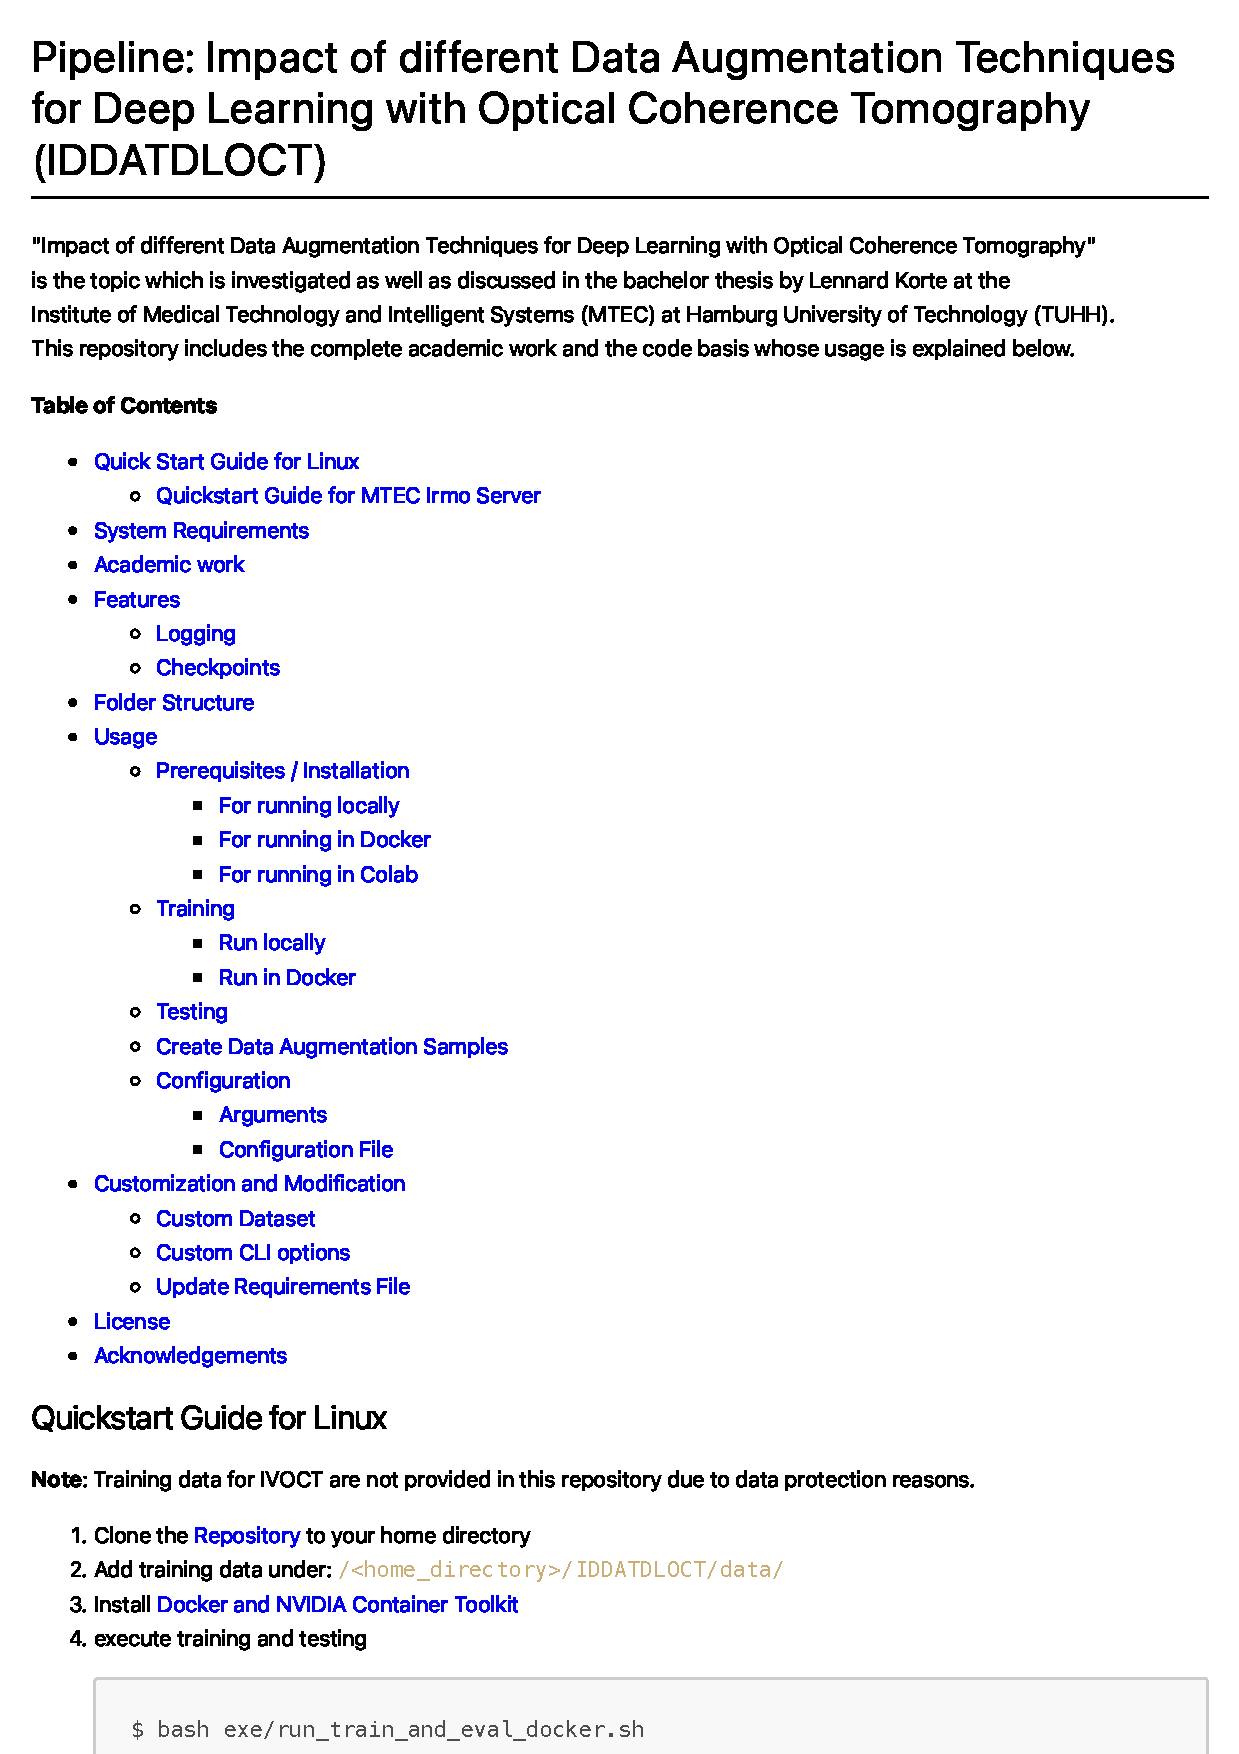
\includepdf[pages={1-},scale=0.8]{./README.pdf}

\backmatter
%\chapter{Bibliography}
\bibliographystyle{splncs03}
\bibliography{references}

\chapter{Declaration}

\thispagestyle{empty}
\begin{center}
	\vspace*{5em}
	
\end{center}
\vspace{2em}
I hereby declare that the work in this thesis was composed and originated independently by myself and has not been submitted for another degree or diploma at any university or other institute. I certify that I have not used any sources or aids other than those indicated.

\vspace{4em}
\begin{minipage}{\linewidth}
	\begin{tabular}{p{15em}p{15em}}
		Date: \today &  .......................................................\\
		& \centering (Signature)\\
	\end{tabular}
\end{minipage}

\end{document}
